\documentclass[a4paper]{report}
\usepackage[utf8]{inputenc}
\usepackage[T1]{fontenc}
\usepackage{RJournal}
\usepackage{amsmath,amssymb,array}
\usepackage{booktabs}

%% load any required packages FOLLOWING this line
\usepackage{color}
\usepackage[table]{xcolor}
\usepackage{fancyvrb}

\usepackage{graphicx}
\usepackage{caption}
\usepackage{subcaption}

\usepackage{booktabs}
\usepackage{multirow}
\usepackage{multicol}

\usepackage{bbm}
\usepackage{amsmath}
\usepackage{amsfonts}

\usepackage{enumitem}
\usepackage{pifont}

\usepackage[algoruled,vlined,linesnumbered]{algorithm2e}
\SetAlFnt{\small}
\SetAlCapFnt{\small}
\SetAlCapNameFnt{\small}


%\renewcommand{\R}{\textsf{\textbf{R}}\xspace}

\renewcommand{\thesection}{\arabic{section}}
\renewcommand{\thesubsection}{\thesection.\arabic{subsection}}
\setcounter{secnumdepth}{2}

\makeatletter
\renewcommand\subsection{\@startsection{subsection}{2}{\z@}%
  {-3.25ex \@plus -1ex \@minus -.2ex}%
  {1.5ex \@plus .2ex}%
  {\normalfont\normalsize\bfseries\boldmath
   \thesubsection\quad}}
\makeatother

\definecolor{magenta}{RGB}{255,0,150}


%\usepackage{Metafix}

\begin{document}


%% do not edit, for illustration only
\sectionhead{Contributed research article}
\volume{18}
\volnumber{2}
\year{2026}
\month{June}
\setcounter{page}{139}



%% replace RJtemplate with your article
\begin{article}
  % !TeX root = RJwrapper.tex
\title{ProfileLadder: Functional-Based Reserving}
\author{by Matúš Maciak, Rastislav Matúš, Ivan Mizera, and Michal Pešta}

\maketitle

\abstract{%
An R package implementing a software environment for predicting loss reserves in insurance, including several novel, nonparametric, and functional-data-based algorithms, is introduced. These algorithms impute incomplete loss development profiles in run-off triangles without relying on traditional parametric assumptions used typically in actuarial practice. The package offers a flexible and computationally effective framework for point-wise and distributional reserve predictions and includes pertinent visualization and diagnostic tools through the S3 methods.
It also provides accessor functions and real-world datasets to support exploratory analysis across insurance, operational risks, and other domains where triangular data structures arise, making modern, transparent, and extensible alternatives to classical approaches accessible in the insurance industry and academic research.
}

\section{Introduction}\label{intro}
One of the key components of insurance practice is maintaining sufficient financial reserves to cover the future claim payments; in non-life insurance, those are often spread into several installments spanning multiple time units (e.g., years). The possibility that an insurance company could default on its payments because of an insolvency caused by business failures is utterly unacceptable; this aspect is closely watched not only by the companies themselves, but also by their regulatory bodies. The companies have to abide by the rules set by the latter, and maintain sufficient funds to cover payments for past and future claims. An example of such a regulatory directive in the European Union is \citet{solvency2}, widely known as "Solvency II".

The insurance environment being inherently stochastic, an important task of actuarial science is to devise stochastic prediction techniques of such loss reserves. An important class of these methods works with aggregated data, organized into a structure known in actuarial science as a run-off triangle. Methods that could be in this context called classical are either quite simple, using so-called development factors (\citealp{Mack1993, Renshaw1998, Clark2003, VD2011}), or rely on parametric assumptions justifying various regression models \citep{Verrall1996, MPO2021}. There is a growing interest in novel methods, offering better predictive performance, transparency, and robustness; 
%\citep{VD2011, PO2014}. 
an R package \CRANpkg{ProfileLadder}, available from CRAN and introduced in this paper, chose to implement those proposed by \cite{MMP2022}. 
%(hereafter MMP).  

Our motivation was and is to create and introduce the R package \CRANpkg{ProfileLadder} as an extension and complement of other packages devoted to claims reserving---most importantly the ground-breaking package  \CRANpkg{ChainLadder} \citep{Rchainladder}, featuring methods for non-life loss reserving that can be considered classical (Mack chain ladder, over-dispersed Poisson and other GLM models, Bornhuetter-Ferguson, etc.). 
%there is also a Python version \citep[\pkg{chainLadder} by][]{Pchainladder}. 
Parametric reserving methods beyond those contained in \CRANpkg{ChainLadder} can be found also in the package \CRANpkg{NetSimR} \citep{NetSimR}. On the other hand, our focus is rather nonparametric, inspired by functional data analysis; also, distributional predictions (which are generally considered compulsory, for instance by Solvency II) are done in this vein: via permutation bootstrap, an original technique introduced by \citet{MMP2022}. Classical techniques typically rely on parametric distributional assumptions, which we are determined to avoid; and our permutation bootstrap technique is applicable also to the classical methods of point prediction (which at the R level means that our \code{permuteReserve()} method can be applied also to the objects generated by \CRANpkg{ChainLadder}).     

Certainly, R is not new to actuarial science: various other topics are covered by packages  \CRANpkg{actuaryr} \citep[][actuarial reporting]{actuaryr}; \CRANpkg{lifecontingencies} \citep[][life contingencies]{JSSv055i10};  \CRANpkg{actuar} and \CRANpkg{actuaRE} \citep[][credibility models]{JSSv025i07,actuaRE}; and others. While \CRANpkg{ProfileLadder} is specifically designed to meet practical needs of actuaries, the methods implemented therein can also be applied in other areas---for instance, to model the spread of infectious diseases, operational risks, or other data where incomplete functional profiles arise. The main methodological outcome, the nonparametric reconstruction of missing fragments of the data, here particularly suited to the structured missingness in run-off triangles, is adaptable also to other domains such as price curves \citep{LieblRameseder}, growth curves \citep{delaigle2013, delaigle2016}, medical data \citep{galmiche2016}, and geological or seismic activity profiles \citep{bauer2021}. 

The paper is organized as follows. Section~\ref{theory} gives a brief summary of the implemented methods, including also some developments that were not available when \citet{MMP2022} was published. In particular, these contributions beyond \citet{MMP2022}, are: a) theoretical---which includes a~methodological approach for a run-off triangle exploratory, adaptation of the MACRAME algorithm beyond its data-driven version, methods for constructing one-year-ahead predictions (a new running diagonal) based on nonparametric approaches and, also, the permutation bootstrap applicable for other than just the functional based prediction methods; and b) practical---mainly in terms of new actuarial datasets with much longer developments than typical and explicit utilization of the proposed methods beyond insurance applications. Section~\ref{Rpackage} describes the main features and implementation details of the \CRANpkg{ProfileLadder} package, in the context of the sample session(s) featuring the main algorithms. Computational efficiency of the functional-based algorithms is illustrated and some comparisons with the classical parametric methods are also given there.  Finally, Section~\ref{beyondSection} provides a~summary and some outlook for possible applications beyond the actuarial context.

\section{Description of the algorithms}\label{theory}
The principal data structure used by claims reserving methods is the so-called run-off triangle. Formally, a \emph{cumulative run-off triangle} is a~dataset $\{Y_{i,j};~i = 1, \dots, n, j = 1, \dots, n + 1 - i\}$, where  $i \in \{1, \dots, n\}$ corresponds to the \emph{occurrence year} (when the insurance event happens) and $j \in \{1, \dots, n + 1 - i\}$ to the \emph{development years} (when the ensuing claims are paid). An example is shown in the left-hand panel of Figure~\ref{fig1}. The gray area exhibits figures which an actuary knows (observes) at a given moment of time; the dots in the white area represent the unknown future, which has to be predicted---the triangle is to be ``completed''. It is assumed that the number of development years in each line is definitive; in particular, the first line of a triangle is already ``completed''---no future payments are expected there. 

%Formally, a \emph{cumulative run-off triangle} %(gray area in Figure~\ref{fig1})
%is a~dataset $\{Y_{i,j};~i = 1, \dots, n, j = 1, \dots, n + 1 - i\}$, where  $i \in \{1, \dots, n\}$ corresponds to the \emph{occurrence year} (when the insurance event happens) and $j \in \{1, \dots, n + 1 - 1\}$ to the \emph{development years} (when the ensuing claims are paid). 

At times, it is also useful to rephrase the same data in terms of an \emph{incremental run-off triangle} $\{X_{i, j};~i = 1, \dots, n; j = 1, \dots, n + 1 - i\}$, with $X_{i, j} = Y_{i, j} - Y_{i, j - 1}$, considering $Y_{i, 0} = 0$. In what follows, random variables denoted by $Y_{i,j}$'s refer to cumulative run-off triangle(s) and random variables denoted by $X_{i,j}$'s to incremental run-off triangle(s). 

The principal starting point of the algorithms proposed by \cite{MMP2022} is the closely related concept of functional development profiles derived from aggregated data or run-off triangles respectively---the concept also known as the ``\emph{patterns of loss emergence}'' \citep[see][]{Clark2003}. Its graphical rendition can be seen in the right-hand panel of Figure~\ref{fig1}. Each point-prediction algorithm provides a~prediction of the overall reserve, the overall future losses/payments, by completing missing fragments within these observed patterns. Given that the structure of the missing values in the run-off triangle is predetermined by its specific form, standard imputation methods assuming missing completely at random (MCAR) situation do not apply (as was theoretically justified by \citealp{MMP2022}). 
\begin{figure}[!t]
        \begin{subfigure}{.615\textwidth} % this sets the figure to be max half the width of the page
            \centering\raisebox{1cm}{
             \scalebox{0.55}{\begin{tabular}{c|>{\centering}p{1.0cm}<{\centering}>{\centering}p{1.0cm}<{\centering}>{\centering}p{1.0cm}<{\centering}>{\centering}p{1.0cm}<{\centering}>{\centering}p{1.0cm}<{\centering}>{\centering}p{1.0cm}<{\centering}>{\centering}p{1.0cm}<{\centering}>{\centering}p{1.0cm}<{\centering}>{\centering}p{1.0cm}p{1.0cm}<{\centering}}
				%\toprule
				\hline
				Accid. & \multicolumn{10}{c}{Development year $j$} \\
				\cline{2-11}
				year $i$ & \cellcolor[gray]{.6} $1$ & \cellcolor[gray]{.6} $2$ & \cellcolor[gray]{.6} $3$ & \cellcolor[gray]{.6} $4$ & \cellcolor[gray]{.6} $5$ & \cellcolor[gray]{.6} $6$ & \cellcolor[gray]{.6} $7$ & \cellcolor[gray]{.6} $8$ & \cellcolor[gray]{.6} $9$ & 
				\cellcolor[gray]{.6} $10$ \\
				\hline
				\cellcolor[gray]{.6}1 & \cellcolor[gray]{.8} 5244  & \cellcolor[gray]{.8}9228 & \cellcolor[gray]{.8}10823 & \cellcolor[gray]{.8}11352 & \cellcolor[gray]{.8}11791 & \cellcolor[gray]{.8}12082 & \cellcolor[gray]{.8}12120& \cellcolor[gray]{.8} 12199 & \cellcolor[gray]{.8}12215 & \cellcolor[gray]{.8}12215\\
				\cellcolor[gray]{.6}2 & \cellcolor[gray]{.8} 5984 & \cellcolor[gray]{.8} 9939 & \cellcolor[gray]{.8}11725 & \cellcolor[gray]{.8}12346 & \cellcolor[gray]{.8}12746& \cellcolor[gray]{.8} 12909 & \cellcolor[gray]{.8}13034 & \cellcolor[gray]{.8}13109& \cellcolor[gray]{.8} 13113 & %13115
                \textcolor{magenta}{\bf .} \\
				\cellcolor[gray]{.6}3 & \cellcolor[gray]{.8} 7452 & \cellcolor[gray]{.8}12421 & \cellcolor[gray]{.8}14171 & \cellcolor[gray]{.8}14752 & \cellcolor[gray]{.8}15066 & \cellcolor[gray]{.8}15354 & \cellcolor[gray]{.8}15637& \cellcolor[gray]{.8} 15720 & 
                % 15744 & 15786
                \textcolor{magenta}{\bf .} & \textcolor{magenta}{\bf .}\\
				\cellcolor[gray]{.6}4 & \cellcolor[gray]{.8}7115 & \cellcolor[gray]{.8}11117 & \cellcolor[gray]{.8}12488& \cellcolor[gray]{.8} 13274 & \cellcolor[gray]{.8}13662& \cellcolor[gray]{.8} 13859 & \cellcolor[gray]{.8}13872& 
                %13935 &13973& 13972
                \textcolor{magenta}{\bf .} & \textcolor{magenta}{\bf .} & \textcolor{magenta}{\bf .}\\
				\cellcolor[gray]{.6}5 & \cellcolor[gray]{.8}5753 & \cellcolor[gray]{.8} 8969  & \cellcolor[gray]{.8}9917 & \cellcolor[gray]{.8}10697 & \cellcolor[gray]{.8}11135 & \cellcolor[gray]{.8}11282 &
                % 11255& 11331& 11332 &11354
                \textcolor{magenta}{\bf .} & \textcolor{magenta}{\bf .} & \textcolor{magenta}{\bf .} & \textcolor{magenta}{\bf .}\\
				\cellcolor[gray]{.6}6 & \cellcolor[gray]{.8}3937 & \cellcolor[gray]{.8} 6524 & \cellcolor[gray]{.8} 7989 & \cellcolor[gray]{.8} 8543 & \cellcolor[gray]{.8} 8757 &
                % 8901 & 9013 & 9012 & 9046 & 9164
                \textcolor{magenta}{\bf .} & \textcolor{magenta}{\bf .} & \textcolor{magenta}{\bf .} & \textcolor{magenta}{\bf .} & \textcolor{magenta}{\bf .}\\
				\cellcolor[gray]{.6}7 & \cellcolor[gray]{.8}5127 & \cellcolor[gray]{.8} 8212 & \cellcolor[gray]{.8} 8976 & \cellcolor[gray]{.8} 9325 & 
                %9718 & 9795 & 9833 & 9885 & 9816 & 9815
                \textcolor{magenta}{\bf .} & \textcolor{magenta}{\bf .} & \textcolor{magenta}{\bf .} & \textcolor{magenta}{\bf .} & \textcolor{magenta}{\bf .} & \textcolor{magenta}{\bf .}\\
				\cellcolor[gray]{.6}8 & \cellcolor[gray]{.8}5046 & \cellcolor[gray]{.8} 8006 & \cellcolor[gray]{.8} 8984 & 
                % 9633 &10102& 10166 &10261 &10252 &10252 &10252
                \textcolor{magenta}{\bf .} & \textcolor{magenta}{\bf .} & \textcolor{magenta}{\bf .} & \textcolor{magenta}{\bf .} & \textcolor{magenta}{\bf .} & \textcolor{magenta}{\bf .} & \textcolor{magenta}{\bf .}\\
				\cellcolor[gray]{.6}9 & \cellcolor[gray]{.8}5129 & \cellcolor[gray]{.8} 8202  & 
                % 9185 & 9681 & 9951& 10033 &10133 &10182 &10182& 10183
                \textcolor{magenta}{\bf .} & \textcolor{magenta}{\bf .} & \textcolor{magenta}{\bf .} & \textcolor{magenta}{\bf .} & \textcolor{magenta}{\bf .} & \textcolor{magenta}{\bf .} & \textcolor{magenta}{\bf .} & \textcolor{magenta}{\bf .}\\
				\cellcolor[gray]{.6}10 & \cellcolor[gray]{.8}3689 & 
                % 6043 & 6789 & 7089 & 7164 & 7197 & 7253 & 7267 & 7266 & 7266
                \textcolor{magenta}{\bf .} & \textcolor{magenta}{\bf.} & \textcolor{magenta}{\bf.} & \textcolor{magenta}{\bf.} & \textcolor{magenta}{\bf.} & \textcolor{magenta}{\bf.} & \textcolor{magenta}{\bf.} & \textcolor{magenta}{\bf.} & \textcolor{magenta}{\bf.}\\
				\multicolumn{11}{c}{~}\\
				\multicolumn{11}{c}{~}
	   \end{tabular}}}
        \caption{Run-off triangle}
        \label{fig1a}
   \end{subfigure}
    \begin{subfigure}{.38\textwidth} % this sets the figure to be max half the width of the page
            \centering
            \raisebox{-0.25cm}[0pt][0pt]{
        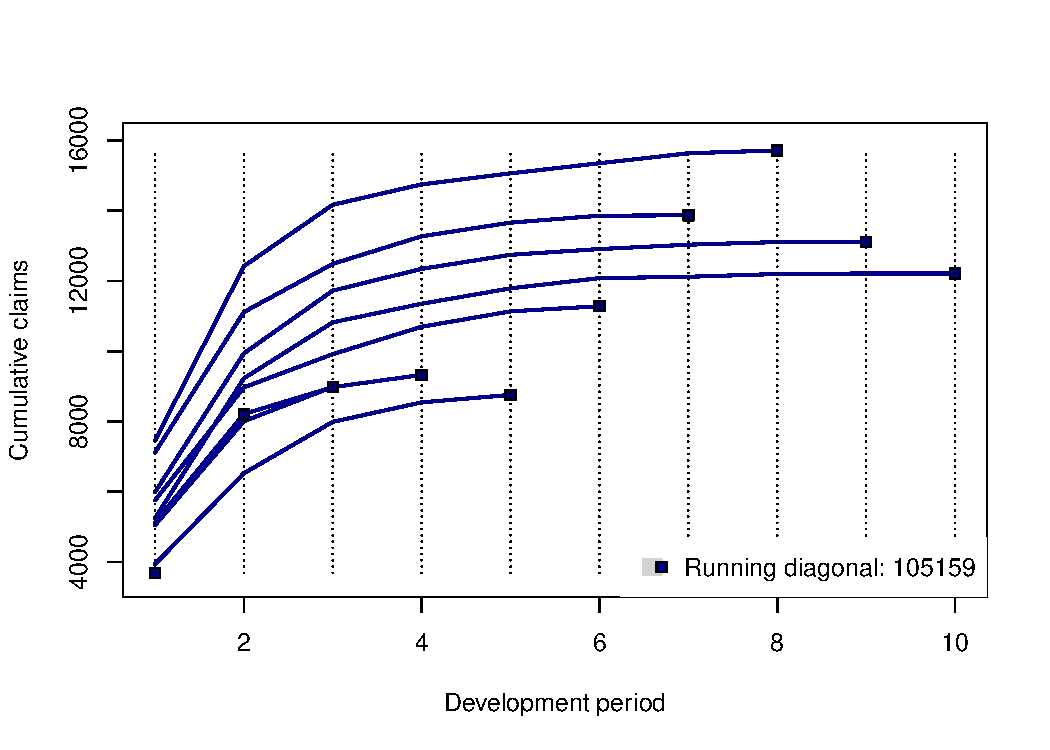
\includegraphics[width=5.5cm]{fig1_B.pdf}
        }
         \caption{Functional profiles}
         \label{fig1b}
    \end{subfigure}   

    \caption{\footnotesize The cumulative run-off triangle (left) of an illustrative portfolio and its incomplete functional development profiles (right). The data, belonging to the Cameron Mutual Insurance Company, are taken from the National Association of Insurance Commissioners (NAIC) database \citep{NAIC2011}. The gray area figures are available to an actuary; the unknown future represented by dots is to be predicted.
    }
    \label{fig1}
\end{figure}

\subsection{PARALLAX {\rm (\textbf{PARALL}el \textbf{A}ppro\textbf{X}imation of missing fragments)}} 
\label{theory_parallax}
The idea of the first algorithm is to impute the missing parts of the run-off triangle by the most similar segments---triangle rows that can be found among the already observed development profiles. The name reflects the fact that in the functional development profiles, the imputation of the missing segments is always performed in a~parallel way.

As described in Algorithm~1 scheme below, each step of the algorithm---the estimation of one unknown/unobserved quantity $Y_{i,j}$ respectively the imputation of one missing linear fragment between the points $[j - 1, Y_{i, j - 1}]$ and $[j, Y_{i,j}]$ for $i = 2, \dots, n$ and $j = n - i + 2, \dots, n$, is performed via the minimization problem in~\eqref{eq2}. The overall reserve prediction  of the true (but unknown) reserve $\mathcal{R}$ (the principal output of the algorithm at the point prediction stage) is 
%\begin{equation}
%\label{def_reserve}
$\widehat{\mathcal{R}} = \sum_{i = 2}^n \widehat{Y}_{i,n} - \sum_{i = 2}^n Y_{i, n + 1 - i}$, 
%\end{equation}
%where the predicted claim payments $\widehat{Y}_{i,j}$ are defined in Algorithm~\ref{alg1}. %\eqref{eq1}. 
which is the difference between the (predicted) ultimate claim payments $\sum_{i = 1}^n \widehat{Y}_{i,j}$ and the claim payments being already settled, the paid amount given by $\sum_{i = 1}^n Y_{i,n + 1 - i}$ (the first row of the run-off triangle is typically assumed to be fully developed and, thus, $Y_{1, n} = \widehat{Y}_{1, n}$).  Besides the reserve estimate $\widehat{\mathcal{R}}$, the algorithm also provides a~full completion of the triangle into an $n \times n$ square---which can be used for a detailed inspection of the overall performance of the algorithm, but, more importantly, it is further needed for the estimation of the whole reserve distribution in terms of the permutation bootstrap resampling, as described in Section \ref{bootstrap}. Note the notation: the $Y_{i,j}$ stand for the observed quantities and $\widehat{Y}_{i,j}$ for the predicted ones.
%Recall, that the input of the algorithm---i.e., the observed run-off triangle, or the development functional profiles respectively---is denoted as $\{Y_{i,j};~i = 1, \dots, n, j = 1, \dots, n + 1 - i\}$ and the completed $n \times n$ square---i.e., the secondary output of the algorithm---is denoted as $\{\widehat{Y}_{i,j};~i = 1, \dots, n, j = 1, \dots, n\}$. 
The algorithm is implemented in the R  function \code{parallelReserve()}; key features and certain implementation details are described in~Section \ref{R_parallaxreact}.

\begin{algorithm}[!htb]%[H]
%\setstretch{1.25}
\caption{PARALLAX}\label{alg1}

{\bf Input: } Observed (cumulative) run-off triangle $\{Y_{i, j}:\,i = 1, \dots, n,\,j = 1, \dots, n+ 1-i\}$\\%[0.2cm]
\Begin{
$\bullet$ Set the observed as the predicted, $\widehat{Y}_{i, j} = Y_{i,j}$ for  $i = 1, \dots, n$ and $j = 1,\dots, n+1-i$\\

\For{$i = 2, \dots, n$}{

\For{$j = n+1-i, \dots, n-1$}{%\smallskip

	$\bullet$ {Find the most similar development profile %$\widehat{\ell}_{i,j} = \arg\min_{\ell \in \{1, \dots, n - j\}} \big| \widehat{Y}_{i, j} - Y_{\ell, j} \big|$}
	\begin{equation}\label{eq2}
		{\widehat{\ell}_{i,j} = \arg\min_{\ell \in \{1, \dots, n - j\}} \left| \widehat{Y}_{i, j} - Y_{\ell, j} \right|}
	\end{equation}}

	$\bullet$ Predict the unobserved (future) value $Y_{i,j+1}$ such that $$\widehat{Y}_{i, j+1} = \widehat{Y}_{i, j} + \big( Y_{\widehat{\ell}_{i,j}, j+1} - Y_{\widehat{\ell}_{i,j} ,j} \big)$$
}   
}

}
%\medskip
{\bf Output: } Completed square $\{\widehat{Y}_{i, j}\}_{i,j = 1}^{n,n}$ and the reserve estimate $\widehat{\mathcal{R}} = \sum_{i = 2}^n \widehat{Y}_{i,n} - \sum_{i = 2}^n Y_{i, n + 1 - i}$ 
\end{algorithm}

\subsection{REACT {\rm (approximation by the most \textbf{RE}cent \textbf{AC}ciden\textbf{T} year)}}
\label{theory_react}
This algorithm  can be viewed as a~simplified version of PARALLAX: instead of looking for the most similar parallel fragment among all existing fragments of the run-off triangle, the REACT algorithm relies---in the spirit of the classical development factors chain ladder methods---on the most recent segment in terms of the previous development year (which is, given the structure of the actuarial data, already observed). Formal description is given in Algorithm~\ref{alg2}. Note that unlike Algorithm~\ref{alg1}, the future payment prediction in Algorithm~\ref{alg2} %\eqref{eq1x} 
is not defined in terms of any minimization problem any more. Therefore, the REACT algorithm is more straightforward and slightly easier to implement; due to evident similarities, both PARALLAX and REACT are implemented within the same R function \code{parallelReserve()}. See Section~\ref{R_parallaxreact}. A comprehensive discussion of various aspects of PARALLAX and REACT, addressing the pros and cons of both algorithms can be found in \cite{MMP2022}, as well as practical user recommendations and guidelines. 

\begin{algorithm}[!htb]%[H]
%\setstretch{1.25}
\caption{REACT}\label{alg2}

{\bf Input: } Observed (cumulative) run-off triangle $\{Y_{i, j}:\,i = 1, \dots, n,\,j = 1, \dots, n+1-i\}$\\%[0.2cm]
\Begin{

$\bullet$ Set the observed as the predicted, $\widehat{Y}_{i, j} = Y_{i,j}$ for  $i = 1, \dots, n$ and $j = 1,\dots, n + 1-i$\\

\For{$i = 2, \dots, n$}{

	\For{$j = n+1-i, \dots, n-1$}{%\smallskip

		$\bullet$ Predict the unobserved (future) value $Y_{i,j+1}$ such that $$\widehat{Y}_{i, j+1} = \widehat{Y}_{i, j} + (\widehat{Y}_{i-1, j+1} - \widehat{Y}_{i - 1, j})$$
}
}

}

{\bf Output: } Completed square $\{\widehat{Y}_{i, j}\}_{i,j = 1}^{n,n}$ and the reserve estimate $\widehat{\mathcal{R}} = \sum_{i = 2}^n \widehat{Y}_{i,n} - \sum_{i = 2}^n Y_{i, n + 1 - i}$ 
\end{algorithm}

Note that for certain run-off triangles, triangles such that $(Y_{i,j} - Y_{i -1, j}) < (Y_{i, j} - Y_{k, j})$ for all $i = 3, \dots, n$, $j = n + 1 - i, \dots, n - 1$, and $k = 1, \dots, i - 2$, both algorithms, PARALLAX and REACT, provide the same reserve prediction and the same completion of the missing fragments: both algorithms are equivalent in such situations. 

\subsection{MACRAME {\rm (\textbf{MA}rkov \textbf{C}hain f\textbf{RA}g\textbf{ME}nt approximation)}}
\label{theory_macrame}
The idea of this algorithm is to utilize a~homogeneous Markov chain (MC) model to obtain the reserve prediction. This strategy is slightly different and more complex than the previous two; despite its additional mathematical complexity, however, it is quite intuitive and can be seen as a~complex but rigorous generalization of the previous two algorithms described above. The underlying stochastic model invites additional user-defined adjustments and practically oriented modifications; unlike the MACRAME algorithm described in \cite{MMP2022}, where only a constrained and rather limited version of the algorithm was proposed, the present implementation in the R function \code{mcReserve()} in \CRANpkg{ProfileLadder} allows for all this fine tuning and adaptations. See Section~\ref{Rmacrame} details.

Firstly, unlike the previous two algorithms, MACRAME is based on the incremental run-off triangle $\{X_{i,j};~i = 1, \dots, n; j = 1, \dots, n + 1 - i\}$. Let us recall that $X_{i,j} = Y_{i,j} - Y_{i, j - 1}$ and $Y_{i, 0} = 0$ for all $i = 1, \dots, n$. In the first step, the algorithm transforms the incremental payments $\{X_{i,j}; i = 1, \dots, n; j = 1, \dots, n + 1 - i\}$ into a finite set  of  states of a~homogeneous Markov chain, $\mathcal{S} = \{s_1, \dots, s_m\}$, and the observed  run-off triangle is used to estimate the matrix of the corresponding transition probabilities $\mathbb{P} = \big(p(s_{\iota_1}, s_{\iota_2})\big)_{\iota_1 = 1, \iota_2 = 1}^{|\mathcal{S}|, |\mathcal{S}|}$, 
for $p(s_{\iota_1}, s_{\iota_2}) = \mathsf{P}[U_{i, j + 1} = s_{\iota_2} | U_{i, j} = s_{\iota_1}]$ where the increment $X_{i, j}$ is represented by the Markov state which is taken by  $U_{i,j}$.  Thus, each row $i \in \{1, \dots, n\}$ is assumed to be governed by an underlying Markov chain process $\{U_{i, j};~j \in \mathbb{N}\}_i$ and these processes are assumed to be independent for $i \in \mathbb{N}$.

The assignment of the observed increments $X_{i,j}$'s into the states in $\mathcal{S}$ is performed via \emph{break points (breaks)}  $- \infty = g_0 < g_1 < \dots < g_{m - 1} < g_m = \infty$; each interval defined by the two adjacent grid points is represented by exactly one state $s_k$ from $\mathcal{S}$). The transformation of the increments $X_{i,j}$'s into the Markov states is then straightforward: if $X_{i, j} \in [g_{k - 1}, g_{k})$ for some $k \in \{1, \dots, m\}$ then $U_{i, j} = s_k$ where $s_{k} \in \mathcal{S}$ and, also, $s_{k} \in [g_{k - 1}, g_{k})$. 

A fully data-driven method for finding appropriate break points $\{g_k\}_{k = 0}^m$ and the corresponding set of Markov states $\mathcal{S} = \{s_1, \dots, s_m\}$ was proposed in \cite{MMP2022}, and it is set as the default option for the \code{mcReserve()} function in the \CRANpkg{ProfileLadder} package. The data-driven method is based on three crucial arguments: 
\begin{itemize}[topsep=0pt, partopsep=0pt, itemsep=0pt, parsep=0pt, labelindent=0pt, leftmargin=18pt]
\item[(i)] to ensure a 1--1 transformation in time and
  the incremental amounts, the default number of Markov states  is the same
  as the number of the development periods, $m = n$;

\item[(ii)] the run-off triangle increments (excluding, by default, the first column of the run-off triangle) denoted as $\{x_{(i+j-3)(i+j-2)/2+i}:=X_{i,j}:\,j>1;\,i+j\leq n+1\}$ are ordered and split into~$m$ bins by using the set of grid points $\{g_m\}_{m = 0}^m$, where 
$g_k:=x_{\left(\left\lceil \frac{kn(n-1)}{2m}\right\rceil+1\right)}$, for $k=1,\ldots,m-1$; 
and, in addition, $g_0 = - \infty$ and $g_m = \infty$;
\item[(iii)] the corresponding Markov states $\mathcal{S} = \{s_1, \dots, s_m\}$ are taken as medians of the increments  belonging to each bin, i.e., $\mathcal{S}:=\big\{s_k:=\mbox{median}(X_{i,j}\in[g_{k-1},g_k):\,j>1,i+j\leq n+1),\,k=1,\ldots,m\big\}$, where the median of an~empty set is omitted (and such bin is not considered).
\end{itemize}
For an illustration of this data-driven principle, consider a small $4 \times 4$ triangle formed 
from the portfolio in Figure~\ref{fig1}. The cumulative triangle is converted into an incremental one 
and all increments (except the first column) are ordered. The third, fourth, and the sixth increments are used to 
define the break points $g_1, g_2$, and $g_3$ as illustrated in the scheme below:
\begin{figure}[!h]
 \begin{subfigure}{.22\textwidth}
    \centering\scalebox{0.55}{{\begin{tabular}{c|cccc}
				\hline
				Accid. & \multicolumn{4}{c}{Development $j$} \\
				\cline{2-5}
				year $i$ & \cellcolor[gray]{.8} $1$ & \cellcolor[gray]{.8} $2$ & \cellcolor[gray]{.8} $3$ & \cellcolor[gray]{.8} $4$ \\

				\cellcolor[gray]{.8}1 &  5244  & 9228 & 10823 & 11352\\
				\cellcolor[gray]{.8}2 & 5984 & 9939 & 11725 & \textcolor{magenta}{\bf .} \\
				\cellcolor[gray]{.8}3 & 7452 & 12421 & 
                \textcolor{magenta}{\bf .} & \textcolor{magenta}{\bf .}\\
				\cellcolor[gray]{.8}4 & 7115 & \textcolor{magenta}{\bf.} & \textcolor{magenta}{\bf.} & \textcolor{magenta}{\bf.}\\[0.1cm]
	   \end{tabular}}}
       \caption{Cumulative triangle}
       \label{fig:ilustration1}
    \end{subfigure} 
    \begin{subfigure}{.08\textwidth}
        \centering\begin{tabular}{l}
             $\longrightarrow$
        \end{tabular}
    \end{subfigure}
    \begin{subfigure}{.22\textwidth}
    \centering\scalebox{0.55}{\begin{tabular}{c|cccc}
				\hline
				Accid. & \multicolumn{4}{c}{Development $j$} \\
				\cline{2-5}
				year $i$ & \cellcolor[gray]{.8} $1$ & \cellcolor[gray]{.8} $2$ & \cellcolor[gray]{.8} $3$ & \cellcolor[gray]{.8} $4$ \\

				\cellcolor[gray]{.8}1 &  5244  & 3984 & 1595 & 592\\

				\cellcolor[gray]{.8}2 &  5984 &  3955 & 1786 & \textcolor{magenta}{\bf .} \\
				\cellcolor[gray]{.8}3 & 7452 & 4946 & \textcolor{magenta}{\bf .} & \textcolor{magenta}{\bf .}\\
				\cellcolor[gray]{.8}4 & 7115 & \textcolor{magenta}{\bf.} & \textcolor{magenta}{\bf.} & \textcolor{magenta}{\bf.}\\[0.1cm]
	   \end{tabular}}
       \caption{Incremental triangle}
       \label{fig:ilustration1}
    \end{subfigure}
    \begin{subfigure}{.08\textwidth}
        \centering\begin{tabular}{c}
             $\longrightarrow$
        \end{tabular}
    \end{subfigure}
     \begin{subfigure}{.38\textwidth}
    \centering\scalebox{0.51}{{\begin{tabular}{l|l}
    \hline
       \cellcolor[gray]{.9} Number of states: & $m = n = 4$ \\[0.1cm]
       \cellcolor[gray]{.9} Ordered increments: & $\{529, 1595, 1786, 3955, 3984, 4969\}$\\[0.1cm]
       \cellcolor[gray]{.9} Break point indexes: & $\left\{\left\lceil \frac{kn(n-1)}{2m}\right\rceil+1;~k = 1,2,3\right\} \equiv \{3,4,6\}$\\[0.2cm]
       \cellcolor[gray]{.9} Break points $\{g_k\}_{k = 0}^4$: & $\{-\infty, 1786, 3955, 4964, \infty\}$\\[0.1cm]
       \cellcolor[gray]{.9} Markov states: & medians of increments in bins $[g_{k - 1}, g_k)$\\[0.1cm]
	   \end{tabular}}}
       \caption{Increments, breaks, and  MC states}
       \label{fig:ilustration1}
    \end{subfigure}
\end{figure}\addtocounter{figure}{-1} %% this is not to be compiled as a figure! 
\vskip-0.4cm
Thus, the resulting Markov states are: $s_1 = 1062$ (i.e., the median of the first two increments, $\{529, 1595\}$, from the first bin, $[-\infty, 1786)$; $s_2 = 1786$ (which is the only increment in the second bin being $[1786, 3955)$); 
$s_3 = 3970$ (again the median of two increments, $\{3955, 3984\}$, from the third bin); and, finally, $s_4 = 4969$ which is the only increment in the last bin---the interval $[g_{3}, \infty)$. The transition matrix is estimated directly by counting the transitions between these four states.

\begin{algorithm}[!htb]%[H]
	%\setstretch{1.25}
		\caption{MACRAME}\label{alg3}
		{\bf Input: } Cumulative run-off triangle $\{Y_{i, j}:\,i = 1, \dots, n,\,j = 1, \dots, n  + 1-i\}$, the sequence of grid points  $\{g_k\}_{k=1}^{m-1}$ (with $g_0:=-\infty$, $g_m:=+\infty$), and the Markov states $\mathcal{S}=\{s_1,\ldots,s_{m}\}$\\%[0.2cm]
		\Begin{
			$\bullet$ Calculate incremental claims $X_{i,j}=Y_{i,j}-Y_{i,j-1}$ for all observed $Y_{i,j}$ (using $Y_{i,0}\equiv 0$)\\
			$\bullet$ Set $\widehat{X}_{i, j} = X_{i,j}$ and $\widehat{Y}_{i, j} = Y_{i,j}$ for  $i = 1, \dots, n$ and $j = 1,\dots, n + 1-i$\\
			$\bullet$ Use the states in $\mathcal{S}$ and transform $\widehat{X}_{i, j}$ into $U_{i, j}$ for $i = 1, \dots, n$ and $j = 1, \dots, n+ 1-i$ such that $U_{i,j}=s$, if $\widehat{X}_{i, j}\in[g_{k-1},g_k)$ and $\mathcal{S}\ni s\in[g_{k-1},g_k)$

			\For{$s_1, s_2 \in \mathcal{S}$}{%\medskip

				$\bullet$ Calculate the transition probability estimates $\widehat{p}(s_1, s_2)$ as
                \begin{equation}
                \label{eq_probs}
  \widehat{p}(s_1, s_2) =
  \frac{\displaystyle\sum_{j=1}^{n-1} \frac{1}{n-j}
    \sum_{i=1}^{n-j}
    \mathbbm{1}{\{ U_{i, j} = s_1, U_{i, j + 1} = s_2\}} }
       {\displaystyle \sum_{j=1}^{n-1} \frac{1}{n-j}
         \sum_{i=1}^{n-j}
         \mathbbm{1}{\{ U_{i, j} = s_1\}} }
\end{equation}
and the estimated transition matrix $\widehat{\mathbb{P}} = \big(\widehat{p}(s_i, s_j)\big)_{i = 1, j = 1}^{m,m}$

			}

			%\medskip
			%$\bullet$ Define the matrix of the estimated transition probabilities $\widehat{\mathbb{P}} = (\widehat{p}(s_1, s_2))_{s_1, s_2 \in \mathcal{S}}$ such that the element $(\widehat{\mathbb{P}})_{k,l}$ stands for $\widehat{p}(y_{k}, y_{l})$, where $k,l \in \{1, \dots, m\}$

			%\medskip

			\For{$i = 2, \dots, n$}{

				\For{$h = 1, \dots, i-1$}{%\medskip 

					$\bullet$ Predict the unobserved value $X_{i,n+1-i + h}$ as $\widehat{X}_{i,n+1-i + h}=\boldsymbol{c}(U_{i,n+1-i})^\top\widehat{\mathbb{P}}^h\boldsymbol{s}$,			
					%				\If{$(\boldsymbol{c}(Y_{i, j}^\circ)^\top\mathbb{P}\boldsymbol{s} = Y_{i, j}^\circ)$}{\medskip 
						%					$\widehat{Y}_{i,j + 1} = \widehat{Y}_{i j}$}
					%				\Else{\medskip 
						%					\begin{equation}\label{eq:M}
							%						\widehat{X}_{i,n+1-i + h} = \boldsymbol{c}(U_{i,n+1-i})^\top\widetilde{\mathbb{P}}^h\boldsymbol{s},
							%					\end{equation}
						where $\widehat{\mathbb{P}}^h \equiv (\widehat{\mathbb{P}})^h$ is the power matrix, $\boldsymbol{s} = (s_1, \dots, s_{m})^\top$, and 
                            $\boldsymbol{c}(U_{i,n+1-i}) = (\mathbbm{1}{\{U_{i,n+1-i}= s_1 \}}, \dots, \mathbbm{1}{\{U_{i,n+1-i} = s_{m}\}})^\top$\\
						%$\bullet$ Transform $\widehat{Y}_{i,j+1}$ into $Y_{i,j+1}^\circ$ as in~\eqref{eq:circ}
						$\bullet$ Compute the corresponding predicted cumulative amount $\widehat{Y}_{i,n+1-i + h}=\widehat{X}_{i,n+1-i + h}+\widehat{Y}_{i,n-i + h}$
					}
				}
			}{\bf Output: } Completed square $\{\widehat{Y}_{i, j}\}_{i,j = 1}^{n,n}$ and the reserve estimate $\widehat{\mathcal{R}} = \sum_{i = 2}^n \widehat{Y}_{i,n} - \sum_{i = 2}^n Y_{i, n + 1 - i}$ 
\end{algorithm}

However, a user can specify the set of states $\mathcal{S} = \{s_1, \dots, s_m\}$ and the breaks $\{g_k\}_{k = 0}^m$ also differently; such alternative settings that lead to various user-defined modifications of the underlying Markov chain process are facilitated via the \code{mcReserve()} function and related functions.
There are various reasons why such modifications could be of interest in practice. For atypical portfolios, standard parametric methods often do not apply: While functional-based techniques are able to handle those, the reserve prediction for portfolios with many zeros and small increments, for instance, would underestimate the true reserve if, particularly, some sudden claim amount increase is expected by actuarial experts (or vice versa). Thus, alternative settings provide useful tuning options for modeling rather atypical situations while also combining them with real expectations.  

Given the set of the Markov chain states in $\mathcal{S}$ one can use the above formula in~\eqref{eq_probs} %from Algorithm~\ref{alg3} 
to construct the empirical estimate $\widehat{\mathbb{P}}$ for the unknown theoretical transition probability matrix $\mathbb{P}$. In some situations (e.g., run-off triangles with extremely short developments---typical for certain portfolios related to material damages, for instance) it may be convenient to exaggerate the state in which the run-off triangle
is already fully developed (i.e., there are only zero increments following after some development period). To this end, a transition probability matrix defined as a convex combination
$\widetilde{\mathbb{P}}:=(1-\delta_n)\widehat{\mathbb{P}}+\delta_n\mathbb{I}_0$ can be used; $\widehat{\mathbb{P}}$ is the estimated transition matrix and $\mathbb{I}_0$ is either a~stochastic matrix with the column corresponding to the state $0\in\mathcal{S}$ consisting of all ones 
and the remaining entries are zeros (if $0\in\mathcal{S}$), or it is a~zero matrix otherwise. The data-driven mixing coefficient  is defined to be
$\delta_n:= 
\frac{1}{n}\sum_{s\in\mathcal{S}}\widehat{p}(s,0)$ if $0\in \mathcal{S}$ and set to zero if $0\notin \mathcal{S}$.

Note that for triangles with not fully developed pay-off profiles (non-zero increments and thus $0 \notin \mathcal{S}$, a common case in~practice), $\delta_n=0$ and therefore the estimate of the transition probability matrix $\widehat{\mathbb{P}}$ in~terms of~\eqref{eq_probs} is used to drive the reserve estimation by the MACRAME algorithm. 

\begin{algorithm}[!tb]%[H]
%\setstretch{1.25}
\caption{Permutation bootstrap}\label{alg4}

{\bf Input: } Completed run-off triangle $\{\widehat{Y}_{i, j}:\,i = 1, \dots, n; j = 1, \dots, n\}$ (output of PARALLAX, REACT, or MACRAME) and the number of permutation bootstrap resamples $B \in \mathbb{N}$ \\
\Begin{
$\bullet$ Standardize the rows in $\{\widehat{Y}_{i, j}\}_{i,j = 1}^n$ to obtain a standardized square $\{\widetilde{Y}_{i,j}\}_{i,j=1}^{n,n}$, where 
\begin{equation}
\label{eq_std}
    \widetilde{Y}_{i,j}:=\widehat{Y}_{i,j}/\widehat{Y}_{i,\ell_i},\quad \ell_i=\min\left\{j\in\{1,\ldots,n\}:\,\widehat{Y}_{i,j}>0\}\right\}
\end{equation}

$\bullet$ Define a set $\Pi(n) = \{\pi^{(b)}\}_{b = 1}^{n!}$ of all distinct permutations of the set $\{1, \dots, n\}$ where $\pi^{(b)}:\,(1, \ldots,n)\mapsto(\pi^{(b)}(1),\ldots,\pi^{(b)}(n))$

\For{$b = 1, \dots, B \leq n!$}{%\smallskip

	$\bullet$ Obtain a permuted square $\{\widetilde{Y}_{\pi^{(b)}(i),j}\}_{i=1,j=1}^{n,n}$, where $\pi^{(b)} \in \Pi(n)$

    $\bullet$ Form the permuted run-off triangle $\{\widetilde{Y}_{\pi^{(b)}(i),j}:\,\pi^{(b)}(i)+j\leq n+1\}$ by omitting the lower-triangular part---values $\widetilde{Y}_{\pi^{(b)}(i),j}$, where $\pi^{(b)}(i) + j > n + 1$

$\bullet$ Estimate the missing fragments in $\{\widetilde{Y}_{\pi^{(b)}(i),j}:\,\pi^{(b)}(i)+j\leq n+1\}$ by using the pertinent algorithm and obtain the bootstrapped completed square $\{\widehat{\widetilde{Y}}_{i,j}:~i= 1, \dots, n; j = 1, \dots, n\}$

    $\bullet$ Apply the back-standardization $\widehat{\widetilde{Y}}_{i,j} := \widehat{\widetilde{Y}}_{i,j} \times  \widehat{Y}_{i, \ell_i}$, for $i,j = 1, \dots, n$

    $\bullet$ Obtain the bootstrapped reserve $\widehat{\mathcal{R}}^{(b)} = \sum_{i = 2}^n \widehat{\widetilde{Y}}_{i,j} - \sum_{i = 2}^n \widehat{Y}_{i, n - i + 1}$
 }   
}
%\medskip
{\bf Output: } Set $\{\widehat{\mathcal{R}}^{(b)}\}_{b = 1}^B$ of bootstrapped reserves mimicking the distribution of interest
\end{algorithm}

\subsection{Distributional predictions: Resampling via permutation bootstrap}
\label{bootstrap}
The reserve prediction $\widehat{\mathcal{R}}$  for the unknown claims reserve $\mathcal{R}$ provides only partial information in the entire loss reserving problem. In practice, a prediction of the whole
reserve distribution is required too (for instance, by risk reserving assessment guidelines like Solvency II). 

Classical techniques employ a residual (parametric or semiparametric) bootstrap approach (typically based on the back-fitted residuals) to emulate the distribution of interest---see, for instance, \cite{EV1999}, \cite{P2003}, or \cite{MMP2022}. However, for the functional-based claims reserving \cite{MMP2022} proposed and theoretically justified a different strategy: permutation bootstrap. The prediction of the reserve distribution is still obtained via bootstrap resampling, but the algorithm avoids the use of residuals by resampling (permuting) the whole functional profiles. The rows of the completed run-off triangle produced by a certain algorithm---by each of those described above, but also any of the classical parametric reserving models implemented in the \CRANpkg{ChainLadder} package---are treated as independent functional profiles. The completed triangle, the data matrix $\{\widehat{Y}_{i,j}\}_{i,j=1}^{n,n}$, can be standardized: each row is divided by the first positive value within the row (considered from the left---which is, very likely, the first incremental payment in each row), as indicated in formula~\eqref{eq_std} in the description of Algorithm 4. The standardization step was proposed by \cite{MMP2022} on the grounds that it is very typical in practice that the claims amounts paid in the first development period substantially increase over the years (possibly the effect of economical growth, inflation, more advanced or more expensive technology, etc.). The standardization is set as a~default, but the user can suppress it if desiring so.

The resulting (standardized) square $\{\widetilde{Y}_{i,j}\}_{i=1,j=1}^{n,n}$ is then resampled \emph{without replacement}, in the~row-wise manner. Formally speaking, for every permutation
$\pi^{(b)}:\,(1\ldots,n)\mapsto(\pi^{(b)}(1),\ldots,\pi^{(b)}(n))$,
where $b=1,\ldots,B$ such that $\pi^{(b)}\neq\pi^{(s)}$ if $b\neq s$, there is a new permuted square $\{\widetilde{Y}_{\pi^{(b)}(i),j}\}_{i=1,j=1}^{n,n}$ and the initial estimation algorithm is applied again to the permuted run-off triangle $\{\widetilde{Y}_{\pi^{(b)}(i),j}:\,\pi^{(b)}(i)+j\leq n+1\}$. After a possible back-standardization, the permuted bootstrap reserve $\widehat{\mathcal{R}}^{(b)}$ is obtained and the set $\{\widehat{\mathcal{R}}^{(b)}\}_{b = 1}^{B}$ is used to estimate the overall reserve distribution. See Algorithm~\ref{alg4}. 

\section{\texorpdfstring{\CRANpkg{ProfileLadder} package for R}{Package for R}}
%\section{\pkg{ProfileLadder} package for R}
\label{Rpackage}
The package provides a toolbox for nonparametric reserving techniques---the reserve point prediction algorithms PARALLAX, REACT, and MACRAME, and the permutation bootstrap algorithm for the prediction of the overall reserve distribution---together with a whole set of tools for handling and preprocessing the data, exploratory analysis, or confirmatory statistical inference. 
A list of key functions is given in Table~\ref{functionslist}; apart from those listed there, the package contains functions (such as \code{plot()}, \code{print()}, or \code{summary()}) corresponding to the (rather standard generic) S3 methods implemented in the package. An integral part of the package are numerous datasets---run-off triangles from actuarial practice, suitable for illustration, validation, and back-testing purposes. 
%In particular, the \textsf{ProfileLadder} package also contains some run-off triangles (not yet made available in any other R package nor any other publicly available source). 
Some of the datasets are unique in this aspect: dataset \code{GFCIB}, provided by the Guarantee Fund of the Czech Insurers’ Bureau (GFCIB) and datasets \code{CZ.casco}, \code{CZ.liability}, and \code{CZ.property} provided by a~major and market-leading insurance company in the Czech Republic contain relatively large (compared to other publicly available actuarial data) run-off triangles (for example, \code{GFCIB} from the mandatory car insurance in the Czech Republic contains $60$ origins/quarters and $60$ development periods---quarters again). 
The triangles represent the claims developments from the beginning of 2008 (1Q) up to the end of 2022 (4Q) while distinguishing four different lines of business---i.e., four portfolios: bodily injuries, material damages, provision payments, and annuities. On the other hand, the datasets \code{CZ.casco}, \code{CZ.liability}, and \code{CZ.property} 
provide separate run-off triangles for gross paid amounts and RBNS reserves (all with the dimensions $18 \times 18$).
For a complete overview refer to the package 
reference manual available on CRAN.

\renewcommand{\arraystretch}{0.9}
\begin{table}[!t]
    \centering
    \scalebox{0.89}{
    \begin{tabular}{ll}
        \toprule
        \textbf{Function name} & \textbf{Function description}\\\midrule
        \code{as.profileLadder()} & function for defining an extended R class \code{profileLadder} to make work \\
        ~ & with the functional development profiles easier and more straightforward\\[0.15cm]
        \code{parallelReserve()} & function that implements two nonparametric, functional-based reserve \\
        ~ & prediction algorithms, PARALLAX and REACT \\[0.15cm]
        \code{mcReserve()} & implements the MACRAME algorithm while also allowing for various\\
         ~ & user-based modifications and explicitly defined  Markov Chain process\\[0.15cm]
         \code{permuteReserve()} & function for estimating the overall reserve distribution in terms of the \\
         & permutation bootstrap (for parametric and nonparametric reserving)\\[0.15cm]
        \code{incrExplor()}  &  provides an exploratory analysis of the run-off triangle increments \\
        ~ & in order to set the Markov chain states and breaks for \code{mcReserve()}\\[0.15cm]
        \code{mcBreaks()} & function to access the break points $\{g_k\}_{k = 0}^m$ used to define the bins\\
         ~ & for the run-off triangle increments  in the \code{mcReserve()} function \\[0.15cm]

         \code{mcStates()} & function to access the Markov chain states $\mathcal{S} = 
         \{s_1, \dots, s_m\}$ representing \\
         ~ & the bins with the run-off triangle increments in the \code{mcReserve()} function\\[0.15cm]
         \code{mcTrans()} & function to access the estimated transition probability matrix $\widehat{\mathbb{P}}$\\
         ~ &  used by the MACRAME algorithm implemented in \code{mcReserve()}\\
        \bottomrule
    \end{tabular}}
    \caption{\footnotesize  Brief descriptions of the key functions in the R package \CRANpkg{ProfileLadder}. More complex
information can be obtained by using the R help session for each function---e.g., \code{help("as.profileLadder")}. Generic functions---such as \code{plot()}, \code{predict()}, \code{print()}, or \code{summary()} used for specific S3 method classes---are not provided in the table.}
    \label{functionslist}
\end{table}

\subsection{PARALLAX and REACT}
\label{R_parallaxreact}
Algorithms PARALLAX and REACT are similar and relatively straightforward. The same also applies for the \code{parallelReserve()} function that implements both these algorithms. Using the illustrative data from Figure~\ref{fig1}, the reserve prediction provided by the PARALLAX or REACT algorithm can be obtained by the R commands
\begin{example}
    R> library("profileLadder")
    R> data(CameronMutual, package = "profileLadder")

    R> parallax <- parallelReserve(CameronMutual, method = "parallax")
    R> react <- parallelReserve(CameronMutual, method = "react", residuals = TRUE)
\end{example}
The PARALLAX algorithm is used as the default option in \code{parallelReserve()} and, therefore, no specification in terms of \code{method = "parallax"} is actually needed. The output of the \code{parallelReserve()} function is a~list (of the {S3} method class \code{profileLadder}) with a~few different  elements (for a comprehensive description of all items we  refer to the R help session that can be obtained in a standard way by typing \code{help("parallelReserve")}). Nevertheless, the most important part of the output is the predicted reserve $\widehat{\mathcal{R}}$ (the list element \code{\$reserve}) and the full completed run-off triangle---contained in the list element \code{\$FullTriangle} (note the analogy with the \CRANpkg{ChainLadder} package). Both pieces of information are automatically provided  by the \code{print()} method as the output:
\begin{example}[commandchars=\\\{\}]
    R> parallax 

    PARALLAX Reserving 
       Estimated Reserve   Estimated Ultimate   Paid Amount   True Reserve 
                    8540               113699        105159           7963

    \textcolor{magenta}{PARALLAX method (functional profile completion)}
           dev
    origin    1     2     3     4     5     6     7     8     9    10
        1  5244  9228 10823 11352 11791 12082 12120 12199 12215 12215
        2  5984  9939 11725 12346 12746 12909 13034 13109 13113 \textcolor{magenta}{13113}
        3  7452 12421 14171 14752 15066 15354 15637 15720 \textcolor{magenta}{15724 15724}
        4  7115 11117 12488 13274 13662 13859 13872 \textcolor{magenta}{13947 13951 13951}
        5  5753  8969  9917 10697 11135 11282 \textcolor{magenta}{11320 11399 11415 11415}
        6  3937  6524  7989  8543  8757  \textcolor{magenta}{8904  8942  9021  9037  9037}
        7  5127  8212  8976  9325  \textcolor{magenta}{9539  9686  9724  9803  9819  9819}
        8  5046  8006  8984  \textcolor{magenta}{9333  9547  9694  9732  9811  9827  9827}
        9  5129  8202  \textcolor{magenta}{8966  9315  9529  9676  9714  9793  9809  9809}
        10 3689  \textcolor{magenta}{6276}  \textcolor{magenta}{7741}  \textcolor{magenta}{8295}  \textcolor{magenta}{8509}  \textcolor{magenta}{8656}  \textcolor{magenta}{8694}  \textcolor{magenta}{8773}  \textcolor{magenta}{8789}  \textcolor{magenta}{8789}       
\end{example}
A fancy version of the print method is used by default which is particularly convenient when working with the run-off triangle shaped data---for instance, compare the following (outputs omitted)
\begin{verbatim}
    R> print(as.profileLadder(observed(CameronMutual)), fancy.print = TRUE)
    R> print(as.profileLadder(observed(CameronMutual)), fancy.print = FALSE)
\end{verbatim}
but this option can be either altered by the command \code{set.fancy.print()}---for which we only refer to the R help session for more details---or it can be fully suppressed by using global options by calling the command 
\begin{verbatim}
    R> options(profileLadder.fancy = FALSE)
\end{verbatim}

The overall (predicted) reserve, reported as  \code{Estimated Reserve}, can be also obtained directly from the completed run-off triangle (in the output above) as $\widehat{\mathcal{R}} = \sum_{i = 2}^n \widehat{Y}_{i,n} - \sum_{i = 2}^n Y_{i, n + 1 - i}$. Some additional quantitative characteristics are also provided: \code{Estimated Ultimate} represents the sum of the last column---the ultimate cumulative payment developments $\sum_{i = 1}^{n} \widehat{Y}_{i, n}$; \code{Paid Amount} gives the amount that was already settled by the insurance company---i.e., the sum of the last running diagonal, $\sum_{i = 1}^{n} Y_{i, n + 1 - i}$; Finally, the true reserve (provided only in situations in which a fully observed run-off triangle is available as an input) is reported as \code{True Reserve}. 
Analogous output, however with different predicted reserve (which is $8358$) and different completed profiles, is obtained for the REACT algorithm (explicit output is, for brevity, omitted). 
For a comparison, the reserve prediction for the \code{CameronMutual} run-off triangle provided by the~standard (parametric) over-dispersed Poisson model (ODP) implemented in the R function \code{glmReserve()} from the package \CRANpkg{ChainLadder} is $8601$. Thus, just in terms of the prediction accuracy, both nonparametric methods outperform the classical (benchmark) actuarial approach in this particular case.  

However, note that the REACT algorithm above is fitted with the additional parameter option \code{residuals = TRUE} (which works regardless of the \code{method} choice). This provides a set of residuals in the output. There are actually two  sets of residuals that can be provided in the output (however, not simultaneously) depending on the input triangle type. Standard (incremental) residuals, defined as $X_{i,j} - \widehat{X}_{i,j}$ for $i = 2, \dots, n$ and $j = n - i + 2, \dots, n$, where $X_{i, j}$ is the ``future'' increment (if known) and $\widehat{X}_{i,j}$ is the predicted counterpart, are provided if a~full triangle (data matrix) is available as the input (thus, the ``future'' payments are supposed to be known). On the other hand, if there is a~standard run-off triangle provided as the input, the so-called ``back-fitted'' residuals are calculated using an~approach that is well-known in the actuarial and finance circles as a~\emph{back-fitting} approach (see, for instance, \cite{popescu_suciu} or \cite{MMP2022} for further details). The main idea behind the back-fitted residuals is to use a~flipped\footnote{The flipped run-off triangle is analogous to a transposition. However, unlike the matrix transposition performed with respect to the main diagonal, the flipped matrix is transposed with respect to the second diagonal---mathematically expressed, for a completed square $\{Y_{i,j};~i = 1, \dots, n; j = 1, \dots, n\}$, the ``flipped triangle'' is the square $\{\widetilde{Y}_{i,j};~i= 1, \dots, n; j = 1, \dots, n\}$, where $\widetilde{Y}_{i,j} = Y_{n + 1 - i, n + 1 - j}$.} completed triangle as an~input and to back-predict the run-off triangle by applying the same estimation procedure in~a~reverse manner so to say. Both sets of residuals can be used in a~straightforward way for some further empirical inspection and analysis (which is typically performed and often also required by regulators when applying  classical parametric methods). 

The summary method applied to an R object of the class \code{profileLadder}---the output from the \code{parallelReserve()} function for instance---provides a complex overview (by adopting an~analogous layout as the one already used in the main actuarial R package \CRANpkg{ChainLadder}.  

\begin{Verbatim}[commandchars=\\\{\}]
    R> summary(react)

    REACT reserve prediction (by origins)
              First Latest Dev.To.Date Ultimate IBNR
        2      5984  13113   1.0000000    13113    0
        3      7452  15720   0.9997456    15724    4
        4      7115  13872   0.9937675    13959   87
        5      5753  11282   0.9912142    11382  100
        6      3937   8757   0.9725677     9004  247
        7      5127   9325   0.9528919     9786  461
        8      5046   8984   0.9172963     9794  810
        9      5129   8202   0.8210210     9990 1788
        10     3689   3689   0.4314620     8550 4861
        total 49232  92944   0.9174942   101302 8358

    \textcolor{magenta}{Overall reserve summary}
        Est.Reserve    Est.Ultimate     Paid Amount    True Reserve        Reserve% 
            8358.00       113517.00       105159.00         7963.00            4.96 

    \textcolor{magenta}{Residual summary (standard incremental residuals)}
         Min   1st Q.   Median     Mean   3rd Q.      Max  Std.Er. 
        -719      -49       -1       -9       34      300      143 

    Total number of residuals: 45,  Total number of unique residuals: 41
    Suspicious residuals (using 2sigma rule): 2,  Outliers (3sigma rule): 1
\end{Verbatim}
The first part of the output is basically an analogy of the  output provided by the \code{summary()} function
when being applied to an output of some estimation method implemented in the R package \CRANpkg{ChainLadder} (the Over-dispersed Poisson model in \code{glmReserve()} for instance). It provides a detailed overview of the ultimate payments and the corresponding reserves by origins. 
\begin{verbatim}
    R> library("ChainLadder")
    R> summary(glmReserve(observed(CameronMutual)))

          Latest Dev.To.Date Ultimate IBNR          S.E        CV
    2      13113   1.0000000    13113    0   0.01035287       Inf
    3      15720   0.9992372    15732   12  29.38975320 2.4491461
    4      13872   0.9934116    13964   92  73.46098788 0.7984890
    5      11282   0.9850694    11453  171  96.26787355 0.5629700
    6       8757   0.9688019     9039  282 120.58781735 0.4276164
    7       9325   0.9397360     9923  598 177.57019068 0.2969401
    8       8984   0.8905630    10088 1104 246.00693847 0.2228324
    9       8202   0.7789914    10529 2327 379.54811405 0.1631062
    10      3689   0.4788422     7704 4015 622.22022041 0.1549739
    total  92944   0.9152986   101545 8601 880.66723938 0.1023913
\end{verbatim}
The function \code{observed()} used above (implemented in the package \CRANpkg{ProfileLadder}) 
transforms the full data matrix \code{CameronMutual} into a run-off triangle with the lower-right triangular part containing  \code{NA} values only (as required by the \code{glmReserve()} function). Note that unlike PARALLAX and REACT the ODP model in \code{glmReserve()} imposes a~distributional assumption and, therefore, the estimated standard errors (\code{S.E.}) and coefficients of variation (\code{CV}) can be provided in the output. On the other hand, the summary of the enriched \code{profileLadder} class object provides, in addition,  the first cumulative payments in the first column which is often used by practitioners to assess
the over-time stability of the given portfolio (and, as already mentioned above, it may play some role in the following permutation bootstrap resampling). 

The second part of \code{summary(react)} above provides the same quantitative information about the estimated reserve as before (\code{Estimated Reserve}, \code{Estimated Ultimate}, \code{Paid Amount} and \code{True Reserve}) but, in addition, there is also a quantification of the prediction precision in terms of \code{Reserve\%} defined in \cite{MMP2022}
as 
$$\texttt{Reserve\%} = 100 \times \Big| \frac{\widehat{\mathcal{R}}}{\mathcal{R}} - 1 \Big|.$$ 
Note that the value can be provided only in situations when the true reserve---the lower triangular part---is available. The last part of the summary output refers to (standard or backfitted) residuals---if the residuals are asked for in the output. Analogous summary is also provided for back-fitted residuals that are calculated in situations where only the run-off triangle itself is given as the input---which can be achieved by the \code{observed()} function as
\begin{verbatim}
    R> summary(parallelReserve(observed(CameronMutual), method="react", residuals=TRUE))
\end{verbatim}

The \code{summary()} function can be also used to plot a  histogram of the residuals (using the parameter \code{plotOption = TRUE}) supplemented with a nonparametric estimate of the underlying density. A simple barplot of the paid amount, estimated ultimate, estimated reserve, and the true  reserve is plotted if no residuals are available. 

The R object of the class \code{profileLadder} can be  visualized with a generic \code{plot()} function. Moreover, if the run-off triangle itself is also of the class \code{profileLadder} the \code{plot()} function can be also used to plot the functional profiles of the run-off triangle itself. The R code
\begin{verbatim}
    R> plot(as.profileLadder(CameronMutual))
    R> plot(parallelReserve(CameronMutual))
\end{verbatim}
provides both plots in Figure~\ref{fig2}.  The same functionality of both generic R functions (\code{summary()} and \code{plot()}) is, of course, provided regardless of the prediction method that is used (PARALLAX or REACT) 
when calling the \code{parallelReserve()} function or the MACRAME algorithm implemented in the \code{mcReserve()} function---see below. 

\begin{figure}[!t]
        \begin{subfigure}{.49\textwidth} 
            \centering
            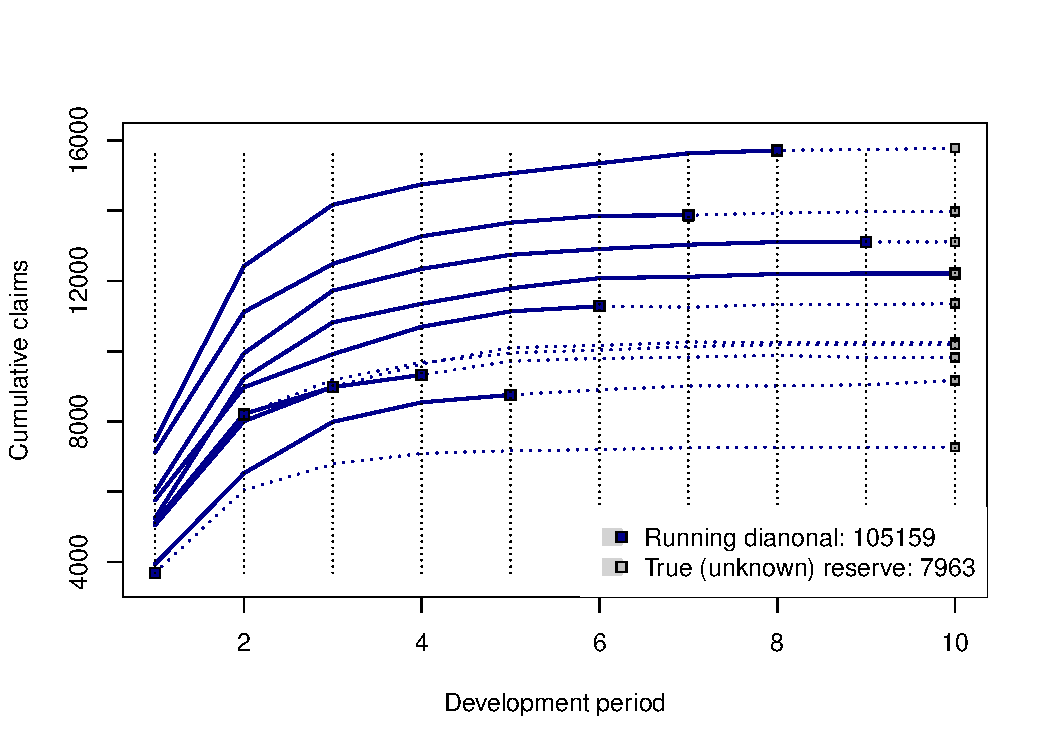
\includegraphics[width = 7.5cm]{fig2_A.pdf}
        \caption{\scalebox{0.8}{\code{plot(as.profileLadder(CameronMutual))}}}
         \label{fig2a}
    \end{subfigure}
    \begin{subfigure}{.49\textwidth} 
            \centering
        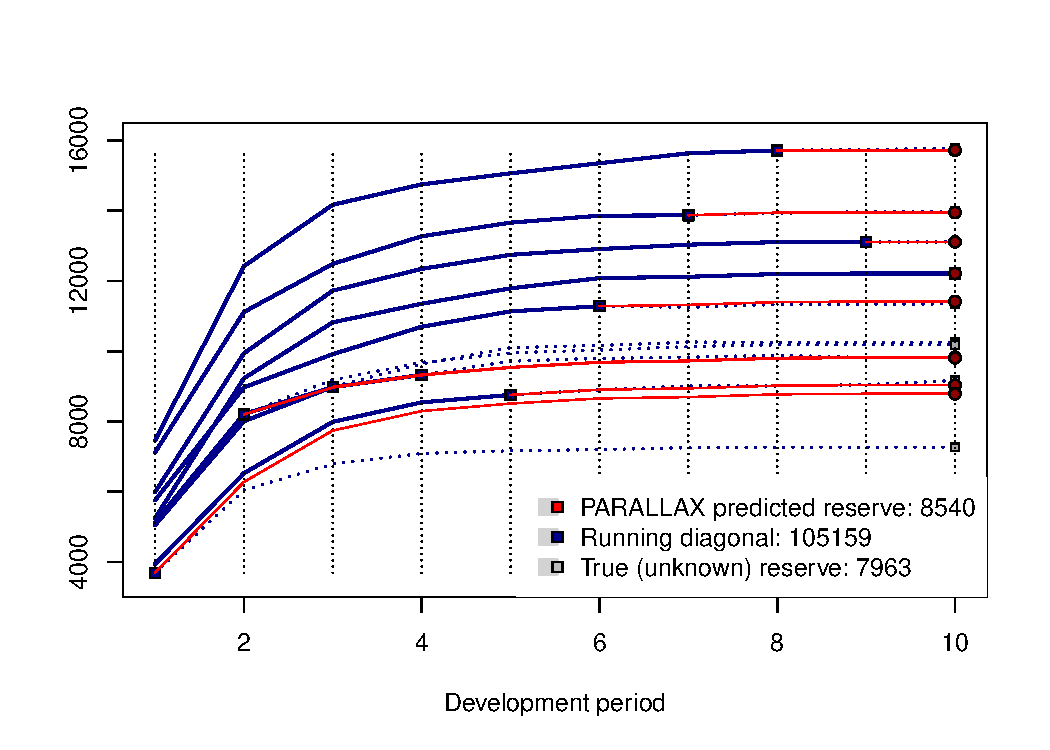
\includegraphics[width = 7.5cm]{fig2_B.pdf}
         \caption{\scalebox{0.8}{\code{plot(parallelReserve(CameronMutual))}}}
         \label{fig2b}
    \end{subfigure}   
    \caption{\footnotesize The observed functional development profiles (blue solid lines) plotted with the  R method \code{plot()} applied to the object of the class \code{profileLadder}. For a 
    "completed" triangle (data matrix), the function also plots the future ``unobserved''  fragments (blue dotted lines) and true ``unknown'' reserve. The predicted functional profiles (red solid lines in the right panel) are provided if \code{plot()} is applied to the output of some \code{parallelReserve()} or \code{mcReserve()}.}
    \label{fig2}
\end{figure}

\subsection{MACRAME}
\label{Rmacrame}
Let us recall that the MACRAME algorithm---as proposed in \cite{MMP2022}---utilizes an~underlying Markov chain mechanism to drive the prediction of the overall reserve $\mathcal{R}$. Due to the data availability (typically there are only 10 -- 15 origin years 
available in run-off triangles in practice which means that there are only about 55 -- 120 incremental payments in total), the underlying Markov chain 
is assumed to be a homogeneous stochastic process. However, there are still relatively many different parameters which need to be properly defined (e.g., the set of the increments, the states of the Markov chain, or the transition probability matrix) and some user-based 
interference can be of some interest here. The MACRAME algorithm, as originally proposed in \cite{MMP2022}, utilizes a fully automatic (data driven) approach to define the set of the Markov chain states $\mathcal{S} = \{s_1, \dots, s_m\}$ and the corresponding break points $\{g_k\}_{k = 0}^m$. Nevertheless, the implementation of the algorithm in the R function \code{mcReserve()} provides users with various  options---starting with a pre-specified  number of the Markov states to be required, selecting the method how the run-off triangle increments are summarized into the states, or even providing a~fully manual specification of the states  $\mathcal{S} = \{s_1, \dots, s_m\}$, breaks $\{g_k\}_{k = 0}^m$, or a subset of increments to be considered. These options are all summarized in Table~\ref{macrame_setting}. The default performance of the \code{mcReserve()} function corresponds with the data-driven selection of the states and breaks---in line with the original MACRAME algorithm proposed in~\cite{MMP2022}. 
Considering again the \code{CameronMutual} dataset, the  MACRAME predicted reserve is obtained by
\begin{verbatim}
    R> macrame <- mcReserve(CameronMutual)
\end{verbatim}
The output of the \code{mcReserve()} function is again the R object of the class \code{ProfileLadder} and it is analogous to the output of the \code{parallelReserve()} function already described before. For brevity, we omit repeating the same details again.  However, specific information related to the underlying Markov chain in the MACRAME algorithm can be also obtained by using various Markov chain (mc) accessor functions (\code{mcBreaks()}, \code{mcStates()}, or \code{mcTrans()}). For instance, 
\begin{verbatim}
    R> mcBreaks(macrame)
      [1]   -Inf   75  147  288  388  554  780 1465 2587 3955  Inf
\end{verbatim}
provides the (default) set of break points $\{g_k\}_{k = 0}^m$ and
\begin{verbatim}
    R> mcStates(macrame)
      [1]   13.0   81.0  197.0  302.5  438.0  601.0  948.0 1672.5 3073.0 3993.0
\end{verbatim}
gives the (default) set of the corresponding Markov chain states $\mathcal{S} = \{s_1, \dots, s_m\}$ such that exactly one state lies between two consecutive break points. The estimate of the transition matrix $\widehat{\mathbb{P}}$ can be obtained by 
\begin{verbatim}
    R> mcTrans(macrame)
             [,1]   [,2]   [,3]   [,4] [,5] [,6] [,7] [,8] [,9] [,10]
      [1,] 0.5000 0.5000 0.0000 0.0000 0.00 0.00 0.00 0.00    0     0
      [2,] 0.6667 0.3333 0.0000 0.0000 0.00 0.00 0.00 0.00    0     0
      [3,] 0.3333 0.6667 0.0000 0.0000 0.00 0.00 0.00 0.00    0     0
      [4,] 0.3333 0.0000 0.3333 0.3333 0.00 0.00 0.00 0.00    0     0
      [5,] 0.0000 0.0000 0.6000 0.2000 0.20 0.00 0.00 0.00    0     0
      [6,] 0.0000 0.0000 0.2500 0.5000 0.25 0.00 0.00 0.00    0     0
      [7,] 0.0000 0.0000 0.0000 0.0000 0.50 0.00 0.50 0.00    0     0
      [8,] 0.0000 0.0000 0.0000 0.0000 0.25 0.75 0.00 0.00    0     0
      [9,] 0.0000 0.0000 0.0000 0.0000 0.00 0.25 0.50 0.25    0     0
     [10,] 0.0000 0.0000 0.0000 0.0000 0.00 0.00 0.25 0.75    0     0
        \end{verbatim}
Generic functions \code{plot()} and \code{summary()} can be both applied to the output in the same way as it was done in case of the \code{parallelReserve()} function.  

In order to provide some useful insight into the structure of the incremental run-off triangle and to offer some visual inspection for various user-based modifications of the underlying Markov chain in the \code{mcReserve()} function, 
there is another software tool implemented in the \CRANpkg{ProfileLadder} package. The R function \code{incrExplor()} takes the run-off triangle as an input (fully observed or not, incremental or cumulative) and returns a complex empirical exploration of the incremental payments.
Recall that the original MACRAME algorithm (as proposed in \cite{MMP2022}) does not take into account the first year payments, values $X_{i,1}$ for $i = 1, \dots, n$, when defining the  grid points $\{g_k\}_{k = 0}^m$ and the corresponding  Markov states in $\mathcal{S}$. The  reason is that most run-off triangles occurring in the real-world actuarial practice have substantially decreasing incremental payment profiles over the consecutive development periods (meaning that $X_{i,j} \to 0$ as $j \to \infty$) and, in order to achieve efficient reserve prediction, it is  more substantial to model 
the tail increments within each row rather than capturing relatively large amounts of the first year (origin) payments.
This can be changed by a user. 

A default functionality of the \code{incrExplor()} function is to provide the data-driven set of bins (the break points respectively) and the corresponding Markov states for the underlying run-off triangle. The first year payments are not considered (i.e., \code{out = 1} is used by default). Taking the \code{CameronMutual} dataset again, the function provides the following output: 
\begin{Verbatim}[commandchars=\\\{\}]
    R> print(runoff.exploratory <- incrExplor(CameronMutual, out = 1))

    \textcolor{magenta}{Data-driven (default) setting of the Markov Chain in MACRAME}
      MC States: 13 81 197 302.5 438 601 948 1672.5 3073 3993

    \textcolor{magenta}{Corresponding bins for the run-off triangle increments}
      [1] "[-Inf, 75)"   "[75, 147)"    "[147, 288)"   "[288, 388)"   "[388, 554)"   
      [6] "[554, 780)"   "[780, 1465)"  "[1465, 2587)" "[2587, 3955)" "[3955, Inf)"  
\end{Verbatim}
Note that all Markov states and also the bins for incremental payments correspond  with the Markov states and the breaks already obtained by \code{mcStates()} and \code{mcBreaks()} from the output of the function \code{mcReserve()}. However, the output from the \code{incrExplor()} function is a complex object of the S3 class \code{mcSetup}. For more details we again refer to the R help session. 
Nevertheless, the summary method applied to the object of the class \code{mcSetup}---the output from \code{incrExplor()} provides the following details: 
\begin{Verbatim}[commandchars=\\\{\}]
    R> summary(runoff.exploratory)
    \textcolor{magenta}{Input triangle type: Cumulative}
    Summary of the increments
                    Min   1st Q.   Median      Mean   3rd Q.  Max   Std.Er.
    Raw increments    0 197.0000 529.0000 1126.0000 1595.000 4969 1340.0000
    Std. increments   0   0.0396   0.1065    0.2267    0.321    1    0.2697

    Total number of increments: 45,  Total number of unique increments: 45
    Number of suspicious increments (using 2sigma rule): 8,  Outliers (3sigma rule): 1

    Data-driven bins for the run-off triangle increments
      [1] "[-Inf, 75)"   "[75, 147)"    "[147, 288)"   "[288, 388)"   "[388, 554)"   
      [6] "[554, 780)"   "[780, 1465)"  "[1465, 2587)" "[2587, 3955)" "[3955, Inf)" 

    Markov Chain states (medians of the increments within each bin)
      [1]   13.0   81.0  197.0  302.5  438.0  601.0  948.0 1672.5 3073.0 3993.0
\end{Verbatim}
Graphical visualization is provided in a standard way using the  \code{plot()} function. Both panels in Figure~\ref{incrExplor1} are produced by the R command
\begin{verbatim}
    R> plot(runoff.exploratory)
\end{verbatim}

\begin{figure}[!t]
    \centering
    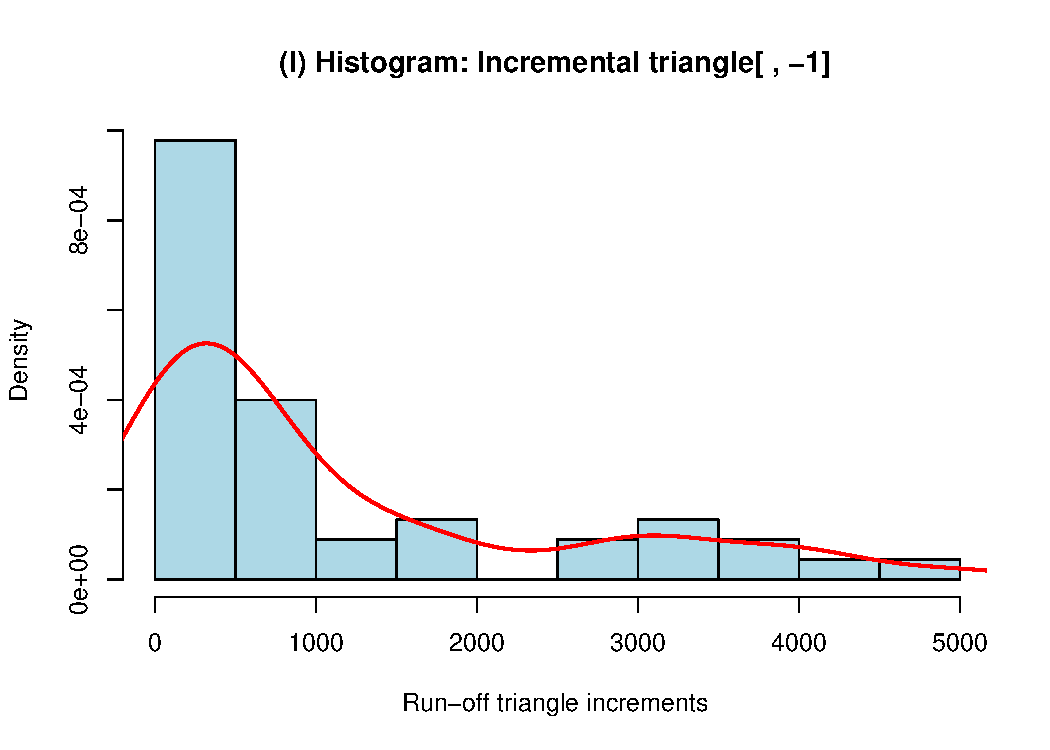
\includegraphics[width = 0.49\textwidth]{fig3_A.pdf}
    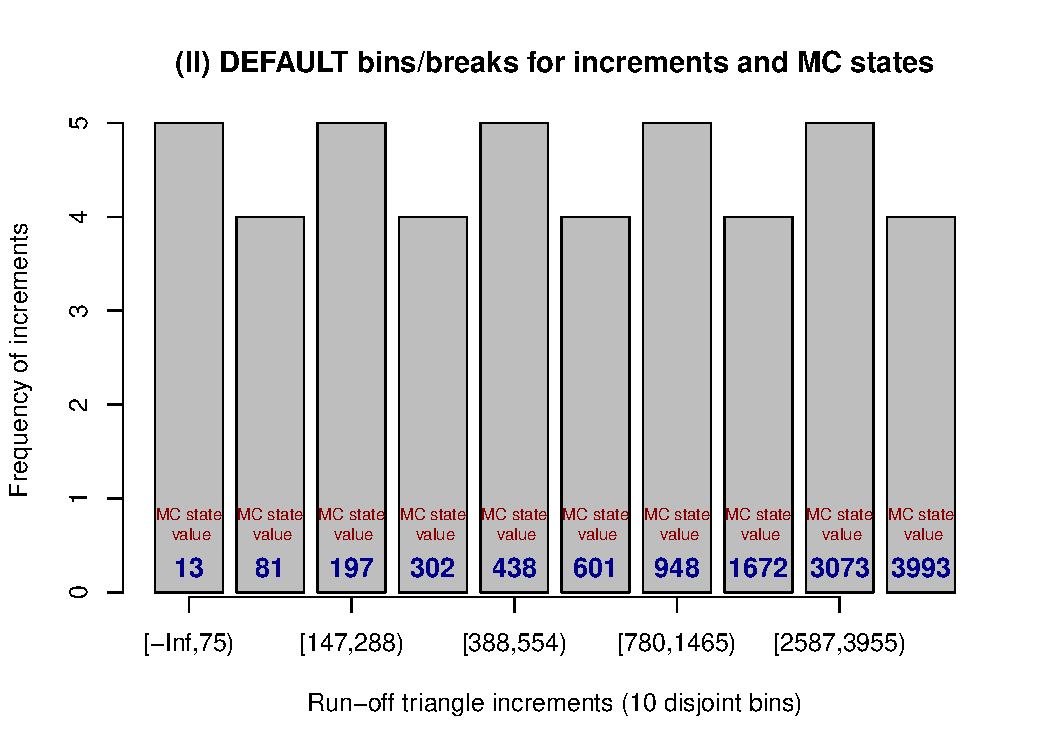
\includegraphics[width = 0.49\textwidth]{fig3_B.pdf}

                \caption{\footnotesize Visualization of the output of the \code{incrExplor()} function when applied to the \code{CameronMutual} dataset. The left-hand panel shows a standard histogram of the run-off triangle increments, values $X_{i, j}$, for $i = 1, \dots, n - 1$ and $j = 2, \dots, n  + 1 - i$. Note that the first year payments $\{X_{i, 1}\}_{i = 1}^n$ are not included. The right-hand panel shows the barplot of the run-off triangle increments distributed across disjoint bins defined by the break points $\{g_{k}\}_{k = 0}^m$, where $g_0 = - \infty$ and $g_m = \infty$. Each bin is represented by the corresponding Markov chain state---blue bold values within the bars.}.             
    \label{incrExplor1}
\end{figure}

If there is a specific interest to also include the first year payments when defining the Markov chain states and the corresponding break points (or, alternatively, to exclude some other columns with the incremental payments), an additional parameter \code{out = 1} can be changed correspondingly---the DEFAULT  value (one) stands for the first year increments 
that are typically not considered; the choice \code{out = 0} uses all available increments $X_{i,j}$, for $i = 1, \dots, n$ and $j = 1, \dots, n + 1 - i$; in order to exclude, for example, first three columns, the parameter can be specified as \code{out = c(1,2,3)}.  The change of this parameter is also reflected by the output of \code{incrExplor()} which, in addition, contains analogous information as before, however, for a user-modified subset of the incremental payments. 
\begin{Verbatim}[commandchars=\\\{\}]
    R> print(runoff.exploratory.all <- incrExplor(CameronMutual, out = 0))
    \textcolor{magenta}{Data-driven (default) setting of the Markov Chain in MACRAME}
    MC States: 13 81 197 302.5 438 601 948 1672.5 3073 3993

    Corresponding bins for the run-off triangle increments
      [1] "[-Inf, 75)"   "[75, 147)"    "[147, 288)"   "[288, 388)"   "[388, 554)"   
      [6] "[554, 780)"   "[780, 1465)"  "[1465, 2587)" "[2587, 3955)" "[3955, Inf)" 

    \textcolor{magenta}{User-modified MC setting}
    MC States: 14.5 125 285.5 400 601 978 2186.5 3689 5007.5 5984

    Corresponding bins for the run-off triangle increments
      [1] "[-Inf, 79)"   "[79, 197)"    "[197, 349)"   "[349, 529)"   "[529, 786)"   
      [6] "[786, 1595)"  "[1595, 3085)" "[3085, 3984)" "[3984, 5244)" "[5244, Inf)" 

    Development periods (run-off triangle columns) not considered: 0
    Method selected to summarize the increments within each bin: DEFAULT (median)
\end{Verbatim}
The \code{summary()} function applied on the  \code{runoff.exploratory.all} object returns analogous information as before but the output  refers to the user-defined subset of increments rather than the default set.  For illustration, Figure~\ref{incrExplor2} is obtained for all run-off triangle increments $\{X_{i,j};~i = 1, \dots n, j = 1, \dots, n + 1 - i\}$, using the R command
\begin{verbatim}
    R> plot(runoff.exploratory.all)
\end{verbatim}

\begin{figure}[!t]
    \centering
    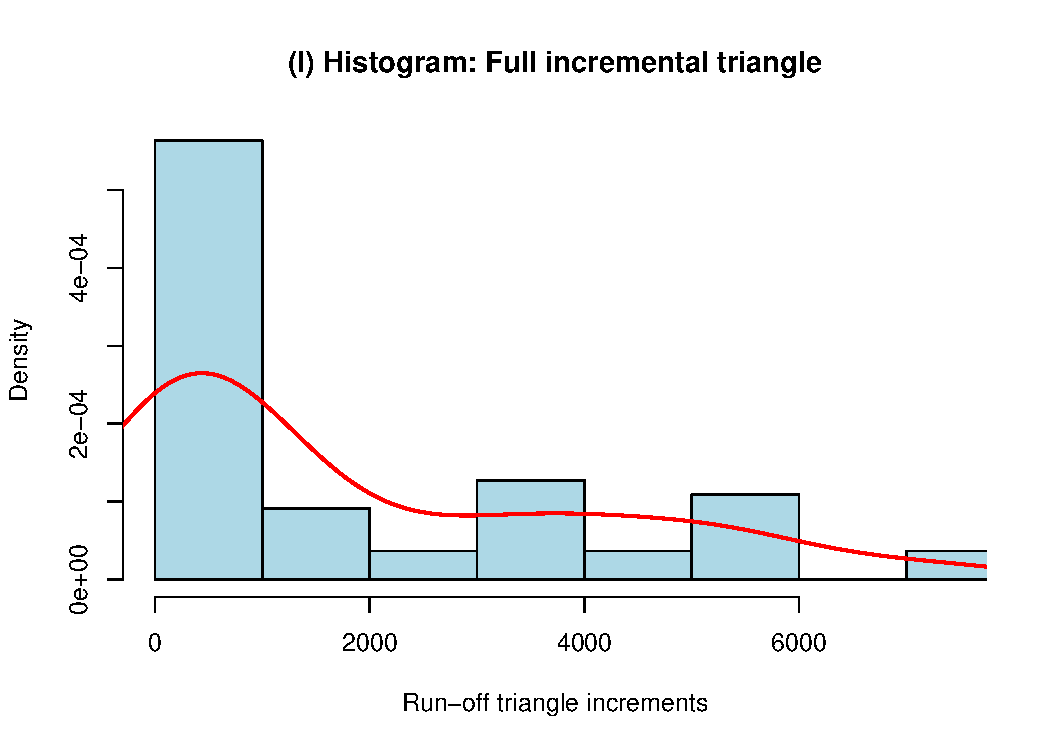
\includegraphics[width = 0.48\textwidth]{fig4_A.pdf}
    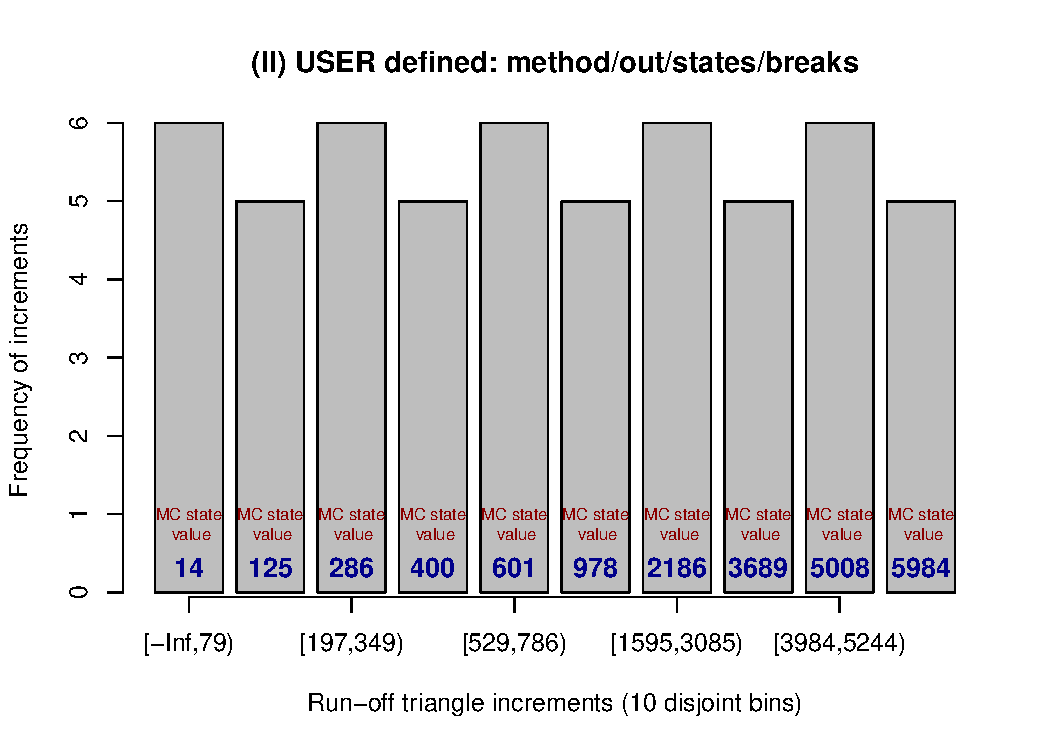
\includegraphics[width = 0.48\textwidth]{fig4_B.pdf}

                \caption{\footnotesize Visualization of the output of the \code{incrExplor()} function when applied to the  \code{CameronMutual} dataset using the additional parameter \code{out = 0}. Instead of the default subset of 45 incremental payments summarized in the panels there are all 55 increments summarized in the same manner.}        
    \label{incrExplor2}
\end{figure}

Note that the Markov chain states and the corresponding break points are also affected by the choice \code{out = 0} and this change is reflected now in Panel~(II) in Figure~\ref{incrExplor2} (compare with the same panel in Figure~\ref{incrExplor1}). The corresponding data-driven Markov states and the breaks are directly accessible by using the accessor methods
\begin{verbatim}
    R> mcBreaks(runoff.exploratory.all)
      [1]   -Inf   79  197  349  529  786 1595 3085 3984 5244  Inf

    R> mcStates(runoff.exploratory.all)
      [1]   14.5  125.0  285.5  400.0  601.0  978.0 2186.5 3689.0 5007.5 5984.0
    \end{verbatim}

Three other parameters can be specified by a user in the \code{incrExplor()} function. The first one is the \code{method} parameter which defines the way how the increments within each bin are summarized to obtain the final Markov state values. By default, the Markov states are calculated as the medians of the increments within each bin (\code{method = "median"}). The method can be changed to the average (\code{method = "mean"}), the minimum increment from the bin (\code{method = "min"}), or the maximum increment respectively (\code{method = "max"}). 

Another parameter that can be used to modify the underlying setting of the Markov chain behind the MACRAME prediction is the parameter \code{states} (which is set to \code{NULL} by default). This parameter sets the Markov states either by 
providing some specific integer value for the number of states (e.g., \code{states = 5}, as in Example~1) while everything else is determined in a data-driven manner proposed in~\citealp{MMP2022} or an~explicit vector of states can be given instead (e.g., \code{states = c(500, 1000, 1500, 2000, 2500)} in Example~2) to enforce not only five states but also their explicit values (with the corresponding break points being the midpoints between the provided states). 

Finally, the last parameter that can be used within the \code{incrExplor()} function  is the \code{breaks} parameter (set to \code{NULL} by default). This parameter can either take the default value \code{NULL} or it can be a~vector of explicit break points $\{g_k\}_{k = 0}^m$. Different combinations of the values of these parameters (\code{states} and \code{breaks} in~particular) result in~different performance of the \code{incrExplor()} function and, consequently, also the \code{mcReserve()} function. For clarity, a~complex description is provided in~Table~\ref{macrame_setting}. The same functionality of the parameters \code{method}, \code{states}, and \code{breaks} also applies when calling the \code{mcReserve()} function to predict the reserve by the MACRAME algorithm. 

\renewcommand{\arraystretch}{0.9}
\begin{table}[!t]
    \centering
    \begin{tabular}{cccc}
        \toprule
        \multicolumn{3}{c}{\bf MACRAME: USER based setting} & \textbf{performance} \\
         ~ & \scalebox{0.8}{\code{states = ... }} & \scalebox{0.8}{\code{breaks = ...}} & \scalebox{0.8}{\code{incrExplor()} \& \code{mcReserve()}}\\\midrule
         ~ & {\code{NULL}} & {\code{NULL}}  & {\scalebox{0.8}{{\bf DEFAULT}~~(fully data-driven)}}\\[0.2cm]
         \multirow{2}{*}{\small\bf 1.} & \multirow{2}{*}{\code{numeric}} & \scalebox{0.9}{any value for} & \scalebox{0.8}{same as DEFAULT (data-driven) }\\[-0.1cm]
         & ~ & \scalebox{0.9}{\code{breaks} is ignored} & \scalebox{0.8}{but the number of states is enforced }\\[0.2cm]
         \multirow{3}{*}{\small\bf 2.} & \multirow{3}{*}{\code{c( ... )}} & \multirow{3}{*}{\code{NULL}} & \scalebox{0.8}{Markov chain states explicitly defined by \code{states = c( ... )}}\\[-0.1cm]
         & & & \scalebox{0.8}{while the corresponding \emph{bins for the run-off increments are}} \\[-0.1cm]
         & & & \scalebox{0.8}{\emph{set as the midpoints between the user-provided states}}\\[0.2cm]
         \multirow{3}{*}{\small\bf 3.} & \multirow{3}{*}{\code{NULL}} & \multirow{3}{*}{\code{c( ... )}} & \scalebox{0.8}{explicit breaks in \code{breaks = c( ... )} are used to form the bins}\\[-0.1cm]
         & & & \scalebox{0.8}{for the increments and the states are obtained by summarizing}\\[-0.1cm]
         & & & \scalebox{0.8}{the increments within each bin by using the \code{method} option}\\[0.2cm]
         \multirow{3}{*}{\small\bf 4.} & \multirow{3}{*}{\code{c( ... )}} & \multirow{3}{*}{\code{c( ... )}} & \scalebox{0.8}{Markov chain states explicitly defined by \code{states = c( ... )}}\\[-0.1cm]
         & & & \scalebox{0.8}{with the \emph{bins for the run-off increments being also user-defined by}}\\[-0.1cm]
         & & & \scalebox{0.8}{\code{breaks = c( ...)} (each bin in \code{breaks} must contain one state )} \\%[-0.2cm]
         \bottomrule
    \end{tabular}
    \caption{\footnotesize User-based modifications for the \code{incrExplor()} and \code{mcReserve()} functions provided by specifying certain values for additional parameters \code{states} and \code{breaks}. Any combination of these two parameters  can be further used with one of four methods for summarizing  the run-off triangle increments within the bins---the default method \code{"median"} or any of \code{"mean"}, \code{"min"}, and \code{"max"} respectively. The modifications 1--4 are illustrated in Examples~1--4.}
    \label{macrame_setting}
\end{table}

In practice, the \code{incrExplor()} function is supposed  to be used to perform a detailed exploratory of various settings of the underlying Markov chain required by the \code{mcReserve()} function. Once the set of breaks  is established and the corresponding Markov states are derived, the output from the \code{incrExplor()} function can be directly forwarded as a~part of the input  for the \code{mcReserve()} function. For illustration, the default performance of the MACRAME algorithm obtained by
\begin{verbatim}
    R> mcReserve(CameronMutual)
\end{verbatim}
and somehow more complex and more explicit specification of the states and breaks---however, all by using the default data-driven approach in the \code{incrExplor()} function---in terms of
\begin{verbatim}
    R> user.states <- mcStates(incrExplor(CameronMutual))
    R> user.breaks <- mcBreaks(incrExplor(CameronMutual))
\end{verbatim}
and directly supplemented into the \code{mcReserve()} function by using the additional parameters \code{states} and \code{breaks} as
\begin{verbatim}
    R> mcReserve(CameronMutual, states = user.states, breaks = user.breaks)
\end{verbatim}
  provide two identical outputs and the same reserve prediction $\widehat{\mathcal{R}}$. For some more detailed illustration of different settings of the \code{incrExplor()} function and, consequently, the \code{mcReserve()} function there are four specific examples provided below together with the corresponding graphical outputs.

\vspace{-10pt}\paragraph{Example 1} Let us start with the simplest  modification that can be used for both the \code{incrExplor()} and \code{mcReserve()} functions (Case~1 in Table~\ref{macrame_setting}). The number of the Markov chain states (by default, the number of states $m \in \mathbb{N}$ is equal to the number of origins, $n \in \mathbb{N}$) can be changed by the parameter \code{states}. In the R code below, there are five Markov chain states specified,  the parameter \code{breaks} is ignored, and the break points and states are derived in a data-driven manner. The following code 
\begin{verbatim}
    R> plot(incrExplor(CameronMutual, states = 5))
    R> plot(mcReserve(CameronMutual, states = 5))
\end{verbatim}
 performs the exploratory analysis of the run-off triangle increments (in terms of the standard output already described above) including the graphical visualization---see Figure~\ref{fig5a}---and, consequently, the reserve is obtained by the \code{mcReserve()} function while using the same five states---see Figure~\ref{fig5b} for the corresponding completed profiles. Note that five Markov chain states are enforced but, otherwise, the run-off triangle increments are summarized analogously---they are split uniformly into five bins and the corresponding Markov  states are obtained by using the median values of the increments within each bin (default method). The predicted reserve is slightly worse than the one obtained by the default setup of the MACRAME algorithm (which gives the predicted reserve roughly $\widehat{\mathcal{R}} = 8082$ while the prediction with only five Markov states produces $\widehat{\mathcal{R}} = 8620$ with the true ``unknown'' reserve being $\mathcal{R} = 7963$). Nevertheless, it can be sometimes useful to manually control (and lower) the amount of the Markov states that are used for the prediction. 

\begin{figure}[!t]
        \begin{subfigure}{.49\textwidth} 
            \centering
            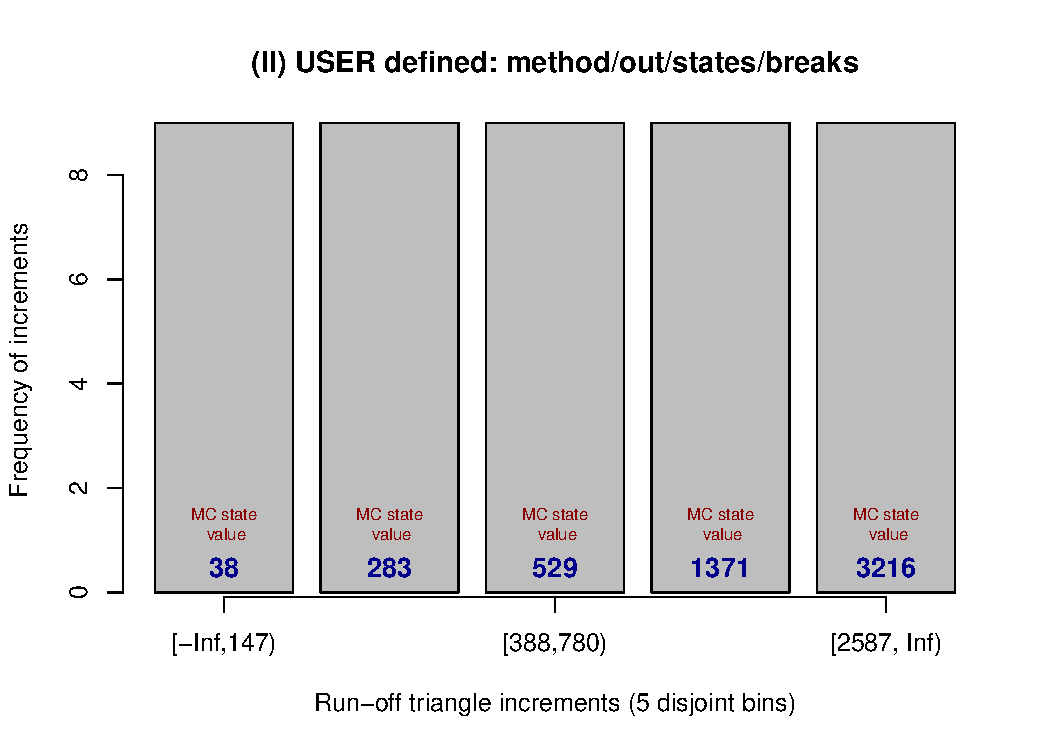
\includegraphics[width = 7.5cm]{fig5_A.pdf}
        \caption{\scalebox{0.8}{\code{plot(incrExplor(CameronMutual, states = 5))}}}
         \label{fig5a}
    \end{subfigure}
    \begin{subfigure}{.49\textwidth} 
            \centering
        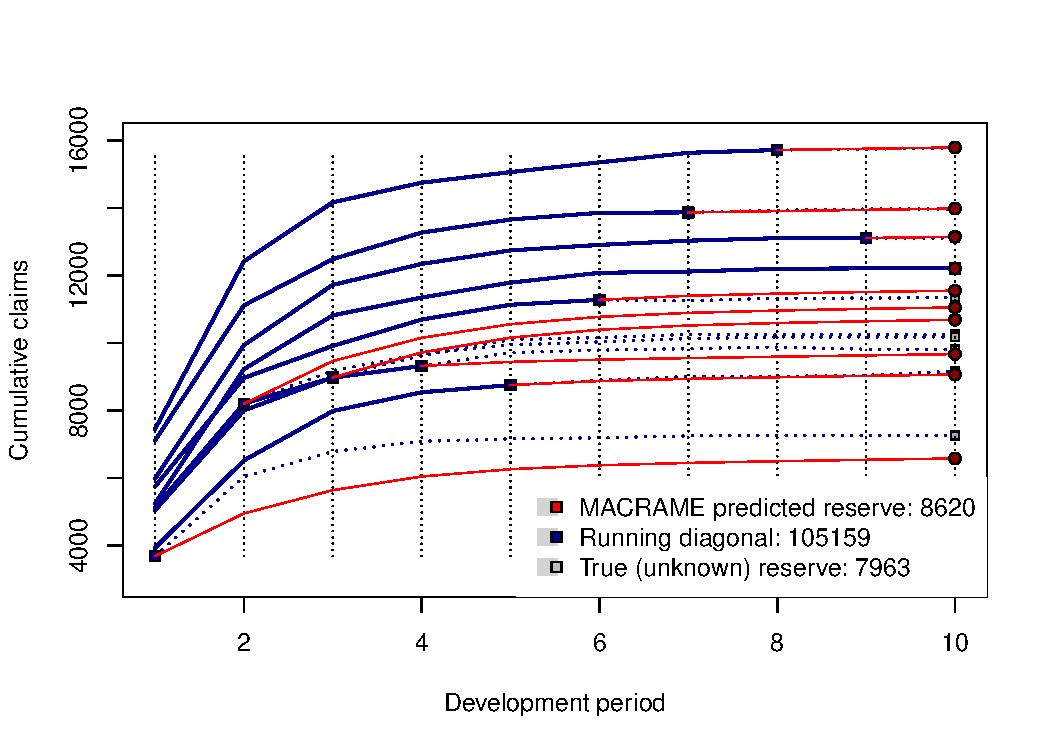
\includegraphics[width = 7.5cm]{fig5_B.pdf}
         \caption{\scalebox{0.8}{\code{plot(mcReseve(CameronMutual, states = 5))}}}
         \label{fig5b}
    \end{subfigure}   
    \caption{\footnotesize Partial plot of the output from \code{incrExplor()} (panel on the left) when applied to the \code{CameronMutual} dataset with the  parameter choice \code{states = 5} (requiring five Markov states to be used). The run-off triangle increments are uniformly distributed into five bins and the corresponding Markov chain states are obtained by the default method---the medians of the increments within each bin are considered. The right panel shows the completed functional profiles provided by MACRAME  with five Markov states used. The figure provides the observed, ``unknown'' future, and completed functional profiles. The predicted reserve, $\widehat{\mathcal{R}} = 8620$, is explicitly reported in the default legend (together with the paid amount and the target ``unknown'' reserve).}
    \label{fig5}
\end{figure}

\vspace{-10pt}\paragraph{Example 2} 
The parameter \code{states} also allows for an explicit definition of the Markov  states for both \code{incrExplor()} and \code{mcReserve()}. 
In such case (Scenario~2 in Table~\ref{macrame_setting}), the corresponding break points $\{g_{k}\}_{k = 1}^{m - 1}$ are defined as the mid-points between the specified state values (which must be all unique). In addition, it holds that $g_0  = - \infty$ and $g_m = \infty$. Similarly as in Example~1, the R code below provides the exploratory analysis of the run-off triangle increments, but instead of specifying just the number of states to be used, explicit Markov chain states are enforced by using \code{states = c(500, 1000, 1500, 2000, 2500)}.
The  MACRAME algorithm uses the same set of states (and breaks) for the consequent reserve prediction. Note that as far as the explicit states are provided, any option of the parameter \code{method = "..."} in the  \code{incrExplor()} function is irrelevant and, therefore, ignored. Analogous graphical outputs provided in Figure~\ref{fig6} are produced by the R commands
\begin{verbatim}
    R> user.states <- c(500, 1000, 1500, 2000, 2500)
    R> plot(incrExplor(CameronMutual, states = user.states))
    R> plot(mcReserve(CameronMutual, states = user.states))
\end{verbatim}
Comparing Figure~\ref{fig5a} (with \code{states = 5}) and Figure~\ref{fig6a} (with \code{states = c(500, 1000, 1500, 2000, 2500)}), it is quite obvious that the numeric specification of the number of states preserves a uniform allocation of the increments in the bins (if possible). However, with the explicit states specification (and the break points $\{g_k\}_{k = 1}^{m - 1}$ being determined as the mid-points between the states) such uniform distribution is not (generally) possible any more and, therefore, relatively large variation is observed among the bars in Figure~\ref{fig6a}.  
\begin{figure}[!t]
        \begin{subfigure}{.49\textwidth} 
            \centering
            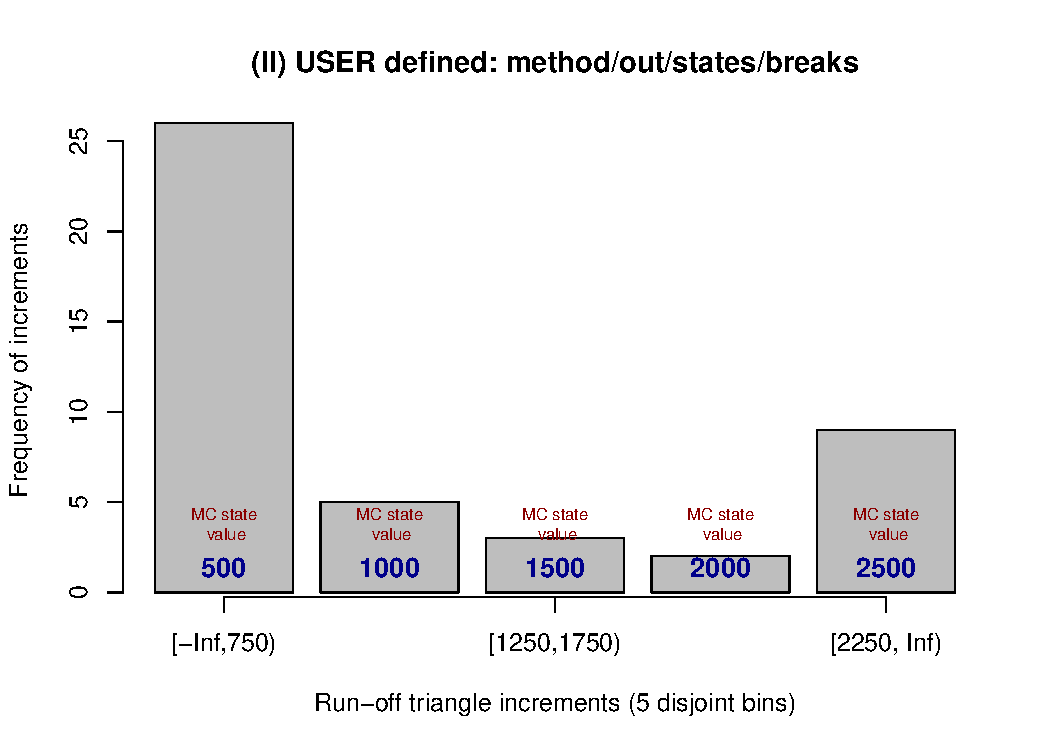
\includegraphics[width = 7.5cm]{fig6_A.pdf}
        \caption{\scalebox{0.8}{\code{plot(incrExplor(CameronMutual, states = user.states))}}}
         \label{fig6a}
    \end{subfigure}
    \begin{subfigure}{.49\textwidth} 
            \centering
        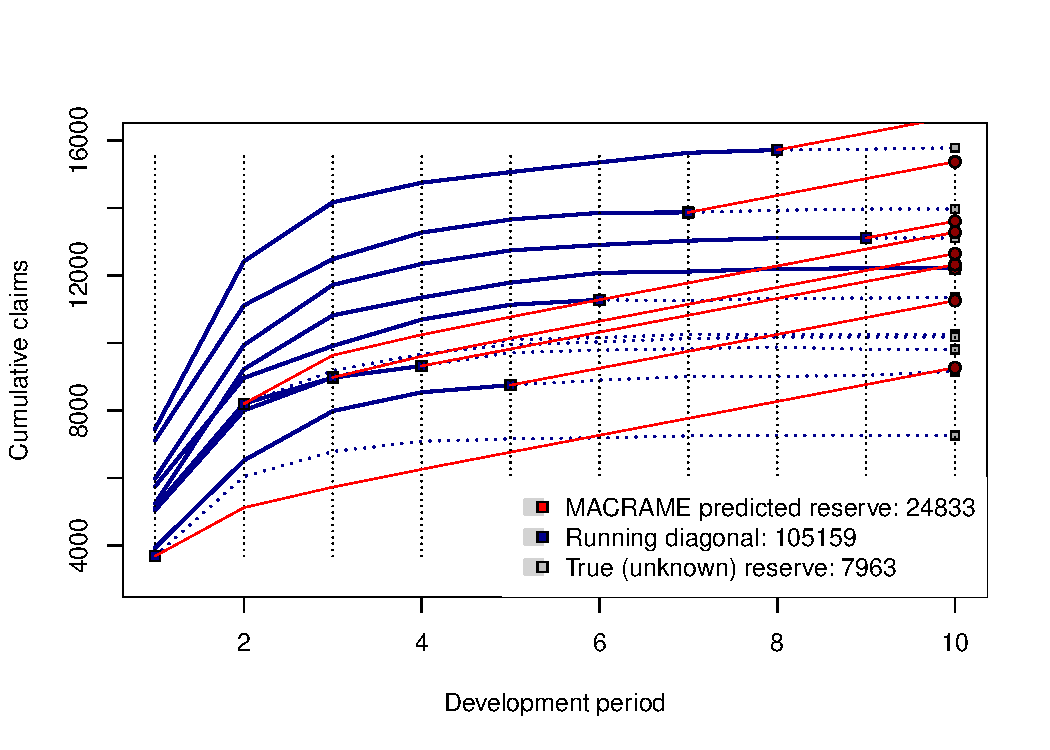
\includegraphics[width = 7.5cm]{fig6_B.pdf}
         \caption{\scalebox{0.8}{\code{plot(mcReseve(CameronMutual, states = user.states))}}}
         \label{fig6b}
    \end{subfigure}   
    \caption{\footnotesize Partial plot of the output from the  \code{incrExplor()} function (left) when applied to the \code{CameronMutual} dataset with an explicit specification of the states---\code{states = c(500, 1000, 1500, 2000, 2500)}. The increments are not distributed uniformly across the bins any more and relatively poor performance of the MACRAME algorithm is also observed in the completed profiles on the right (the predicted reserve heavily overestimates the true reserve due to almost no Markov chain states that would properly model the development tails).}
    \label{fig6}
\end{figure}
The Markov chain states in Figure~\ref{fig6a} (blue bold values within the bars) indeed correspond with the declaration of the states provided by \code{states = c(500, 1000, 1500, 2000, 2500)}. Thus, there are again five bins for the run-off triangle increments but the bins are now more restricted. As a~result, the development tails of the run-off triangle are approximated very roughly (note that there are more than 25 increments in~the first bin) and, therefore, the reserve is (not surprisingly) heavily overestimated (compare Figure~\ref{fig6b} with Figure~\ref{fig5b}).  

\vspace{-10pt}\paragraph{Example 3} Instead of enforcing the Markov chain states one can also pre-specify the set of breaks  $\{g_k\}_{k = 0}^m$ that are used to form the bins for the run-off triangle increments (Case~3 in Table~\ref{macrame_setting}). The corresponding states are obtained by summarizing the increments within the bins (either by using the default median method or by specifying other options with the \code{method} parameter). The following R code uses again five bins  defined by four grid points and the corresponding Markov states are obtained as the medians of the increments within the bins. 
\begin{verbatim}
    R> user.breaks <- c(500, 1000, 1500, 2000)
    R> plot(incrExplor(CameronMutual, breaks = user.breaks))
    R> plot(mcReserve(CameronMutual, breaks = user.breaks))
\end{verbatim}
Both plots are provided in Figure~\ref{fig7}. It is also worth mentioning that if the specified break points $\{g_k\}_{k = 1}^{m - 1}$ define some empty bin with no  increment within the bin, then two neighboring bins are automatically merged in a way that each bin 
contains at least one increment. More formally, if there is no increment in the bin $[g_k, g_{k + 1})$ for some $k \in \{1, \dots, m - 1\}$
then a new bin defined as $[g_{k - 1}, g_{k + 1})$ is used instead. Similarly, if there is no increment in the first bin $(g_0, g_1)$, where $g_0 = -\infty$, then the first bin is re-defined as $(-\infty, g)$, where $g = min_{\{2 \leq k \leq m\}}\{g_k;~g_k > min{\{X_{i,j}:~ 1 \leq i \leq n, 2 \leq j \leq n - i + 1\}}\}$. Thus, it is also possible, for some rather atypical run-off triangles, that there is only one bin used for all  (typically zero) increments (no matter what is specified by \code{states} or \code{breaks}) and the underlying Markov chain process has only one (typically zero) state, i.e., $|\mathcal{S}| = |\{s\}| = 1$.
\begin{figure}[!t]
        \begin{subfigure}{.49\textwidth} 
            \centering
            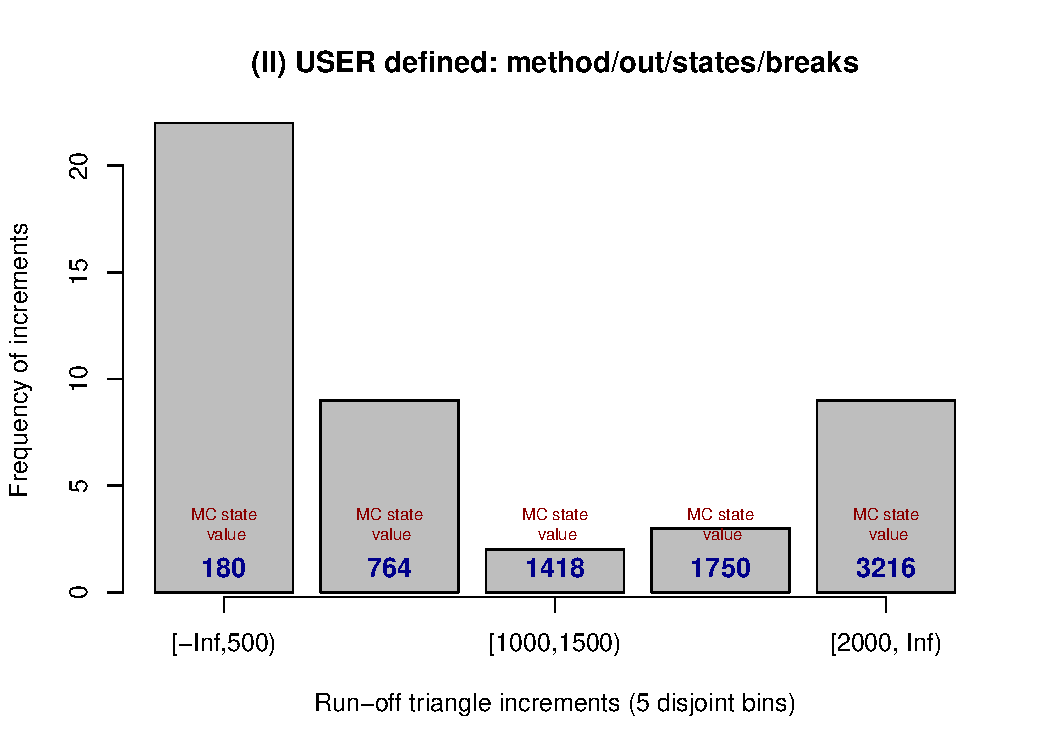
\includegraphics[width = 7.5cm]{fig7_A.pdf}
        \caption{\scalebox{0.8}{\code{plot(incrExplor(CameronMutual, breaks = user.breaks))}}}
         \label{fig7a}
    \end{subfigure}
    \begin{subfigure}{.49\textwidth} 
            \centering
        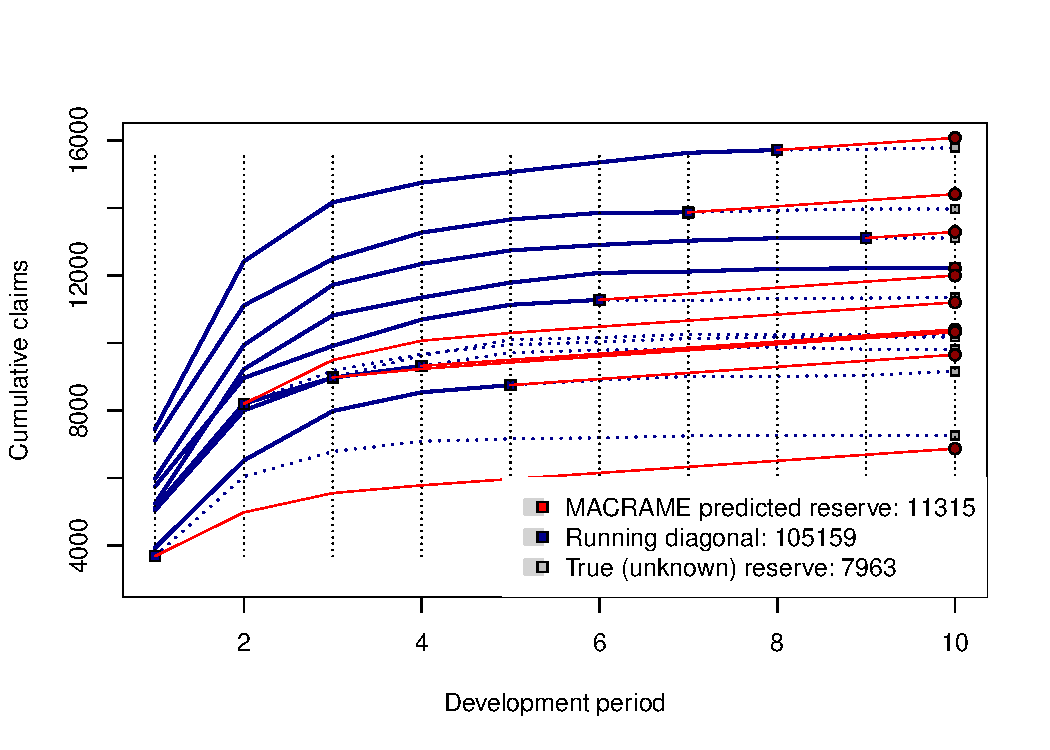
\includegraphics[width = 7.5cm]{fig7_B.pdf}
         \caption{\scalebox{0.8}{\code{plot(mcReseve(CameronMutual, breaks = user.breaks))}}}
         \label{fig7b}
    \end{subfigure}   
    \caption{\footnotesize Partial plot of the output from the \code{incrExplor()} function (left) when applied to the \code{CameronMutual} dataset with an explicit specification of the breaks by using \code{breaks = c(500, 1000, 1500, 2000)}. The corresponding completed profiles are on the right-hand side. The predicted reserve is $\widehat{\mathcal{R}} = 11315$.}
    \label{fig7}
\end{figure}

\vspace{-10pt}\paragraph{Example 4} Finally, we briefly address one more important  modification of the underlying Markov chain. Note that the choice of the summary method (i.e., \code{method = c("median", "mean", "min", "max")}) is only applicable for the \code{incrExplor()} function. The \code{mcReserve()} function only allows one to specify the set of breaks and the set of  states. This is however not limiting in practice.

The R code below specifies the user-based choice for breaks (i.e., \code{breaks = c(500, 1000, 1500, 2000)}) and, also, the user selected method how the increments within each bin are supposed to be summarized (i.e., \code{method = "min"}). The corresponding Markov chain states are calculated by the \code{incrExplor()} function and, together with the pre-specified breaks, they can be both forwarded to the \code{mcReserve()} function by using the \code{mcStates()} accessor and both parameters \code{breaks} and \code{states} (Case~4 in Table~\ref{macrame_setting}).
\begin{verbatim}
    R> user.breaks <- c(500, 1000, 1500, 2000)
    R> user.method <- incrExplor(CameronMutual, breaks = user.breaks, method = "min")

    R> final.states <- mcStates(user.method)
    R> mcReserve(CameronMutual, breaks = user.breaks,  states = final.states)
\end{verbatim}
 The explicit outputs and plots are omitted for brevity. Note that if functions \code{incrExplor()} and \code{mcReserve()} are used with an explicit specification of both the set of breaks\footnote{The set of breaks $\{g_k\}_{k = 1}^{m - 1}$ can be specified differently but for a proper functionality of the MACRAME algorithm it is important that $g_0 = -\infty$ and $g_m = \infty$. The user can however either specify a sequence of breaks in a form $-\infty \neq g_1 < \dots < g_{m - 1} \neq \infty$ and boundary values $g_0 = -\infty$ and $g_m = \infty$ are filled in automatically. Alternatively, the sequence of break points with one or both boundary points can be supplied.}
$\{g_k\}_{k = 1}^{m - 1}$ and  the set of states $\mathcal{S} = \{s_1, \dots, s_m\}$ then the Markov states provided in \code{states = c( ... )} must represent a~valid sequence of unique values such that exactly one state value belongs to exactly one bin determined by the break points $-\infty = g_0 < g_1 < \dots < g_{m - 1} < g_m = \infty$. 

\subsection{Permutation bootstrap}
The third key function implemented in the \CRANpkg{ProfileLadder} package---providing the overall reserve distribution for functional-based reserving methods but also for traditional parametric approaches already available in the \CRANpkg{ChainLadder} package---is the \code{permuteReserve()} function. The function performs the permutation bootstrap for all possible reserving algorithms (e.g., Mack model, Tweedie model, GLM based reserving, PARALLAX, REACT, or MACRAME) with no explicit need to specify which algorithm should be used. The input for the \code{permuteReserve()} function is an output of some reserving algorithm implemented in R and it can be an object of different classes (for instance, \code{glmReserve}, \code{tweedieReserve}, \code{MackChainLadder}, or \code{profileLadder}). The output from the \code{permuteReserve()} function is always the object of the S3 class \code{permutedReserve}. 

 For illustration, the overall reserve distribution for the \code{CameronMutual} dataset---provided by the MACRAME algorithm with $500$ permutation bootstrap resamples can be obtained as
\begin{Verbatim}[commandchars=\\\{\}]
    R> print(distribution.macrame <- permuteReserve(mcReserve(CameronMutual)))
      |>>>>>>>>>>>>>>>>>>>>>>>>>>>>>>>>>>>>>>>>>>>| 100% elapsed=04s
    \textcolor{magenta}{MACRAME based reserving}
       Est.Reserve    Est.Ultimate     Paid Amount    True Reserve 
          8081.963      113240.963      105159.000        7963.000 
    \textcolor{magenta}{Permutation bootstrap (B = 500)}
         Boot.Mean         Std.Er.        BootCov%     BootVar.995 
          9422.290        1457.072          15.464           1.471 
\end{Verbatim}
Two sets of values are listed in the output. The first part corresponds to the point prediction of the overall reserve (also discussed before) and the second part of the output summarizes the overall reserve distribution. The first two values in the second part of the output---the average (\code{Boot.Mean}) over $B \in \mathbb{N}$ bootstrap  reserves $\{\widehat{\mathcal{R}}^{(b)}\}_{b = 1}^B$  and the corresponding standard error (\code{Std.Er.})---provide some basic characterization of the location and shape of the estimated reserve distribution. In addition, two qualitative measures proposed in \cite{MMP2022} are provided for some practical assessment of the resampling performance. The value of \code{BootCov\%} expresses (in percentages) the coefficient of variation of the bootstrap distribution and the value of \code{BootVar.995} gives the $99.5\%$ quantile (by default) of the  distribution relative to the bootstrap mean (other choice of the quantile can be applied by changing the parameter \code{quantile = 0.995}). Both these quantities were defined, explained, and consequently also used for the empirical comparisons in \cite{MMP2022} and more detailed discussion can be also found there. Note that the default quantile level of $0.995$ is explicitly required by the Solvency~II principle.

In general, the \code{permuteReserve()} function returns a complex object of the class \code{permutedReserve} and standard  generic methods (such as the \code{summary()} function or the \code{plot()} function) can be applied to assess more specific details from the object. The summary method provides the following output: 

\begin{Verbatim}[commandchars=\\\{\}]
    R> summary(distribution.macrame)

    MACRAME based reserve prediction (with B = 500 bootstrap permutations)
              First Latest Dev.To.Date   Ultimate       IBNR        S.E        CV
        2      5984  13113   0.9964286  13160.000   47.00000   19.04960 0.4053106
        3      7452  15720   0.9950067  15798.889   78.88889   49.20912 0.6237776
        4      7115  13872   0.9906724  14002.611  130.61111  125.80444 0.9631986
        5      5753  11282   0.9840866  11464.438  182.43827  117.91093 0.6463059
        6      3937   8757   0.9749940   8981.594  224.59362  165.04382 0.7348553
        7      5127   9325   0.9535135   9779.620  454.61986  256.95086 0.5651994
        8      5046   8984   0.8241040  10901.537 1917.53724  495.52130 0.2584155
        9      5129   8202   0.7664369  10701.468 2499.46806  698.02698 0.2792702
        10     3689   3689   0.5915835   6235.806 2546.80632  613.02222 0.2407023
        total 49232  92944   0.9200011 101025.963 8081.96337 1457.07250 0.1802869

    \textcolor{magenta}{Overall reserve distribution}
         Boot.Mean        Std.Er.       BootCov%    BootVar.995 
       9422.289972    1457.072499      15.464102       1.471458

    The MACRAME predicted reserve represents the 15.37% quantile of the distribution
    Bootstrap simulated reserves beyond 2sigma rule: 20 (out of 500)
\end{Verbatim}
In a correspondence with the classical parametric methods, the summary output above now also provides standard errors (\code{S.E}) and coefficients of variation (\code{CV}). The graphical visualization is also  analogous with the classical parametric reserving methods implemented in the \CRANpkg{ChainLadder} package. Figure~\ref{fig10} is obtained by the R command
\begin{verbatim}
    R> plot(distribution.macrame)
\end{verbatim}

    \begin{figure}[!t]
        \begin{subfigure}{.49\textwidth} 
            \centering
            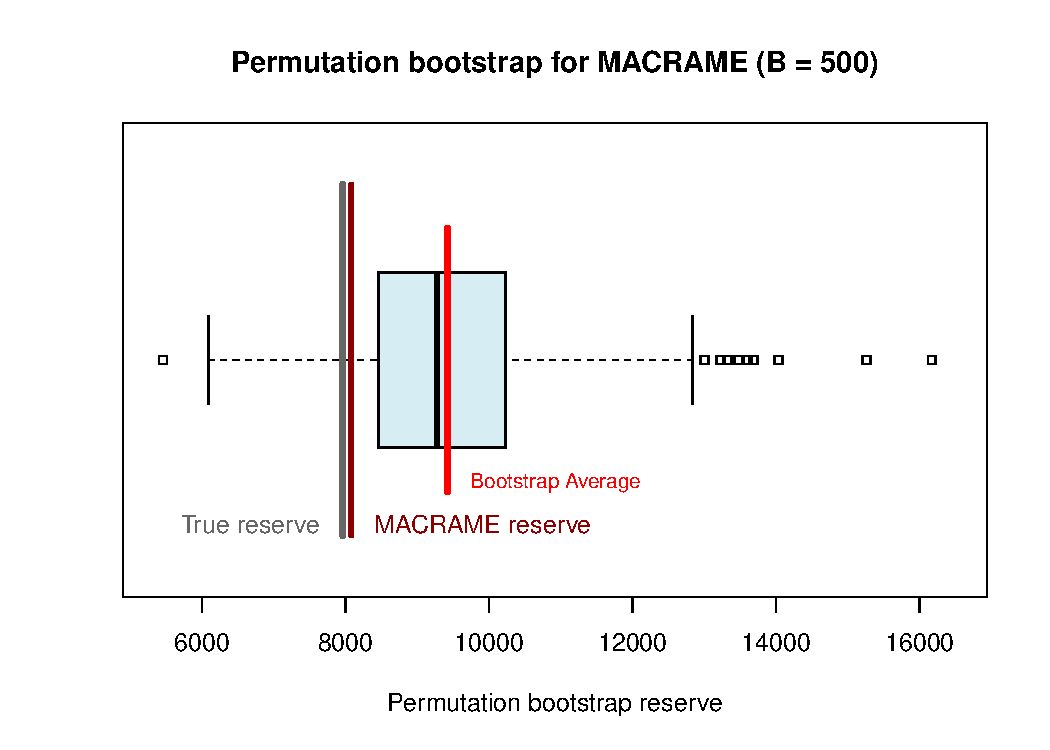
\includegraphics[width = 7.3cm]{fig8_A.pdf}
        \caption{Boxplot of $\{\widehat{\mathcal{R}}^{(b)}\}_{b = 1}^{100}$ values}
         \label{fig10a}
    \end{subfigure}
    \begin{subfigure}{.49\textwidth} 
            \centering
        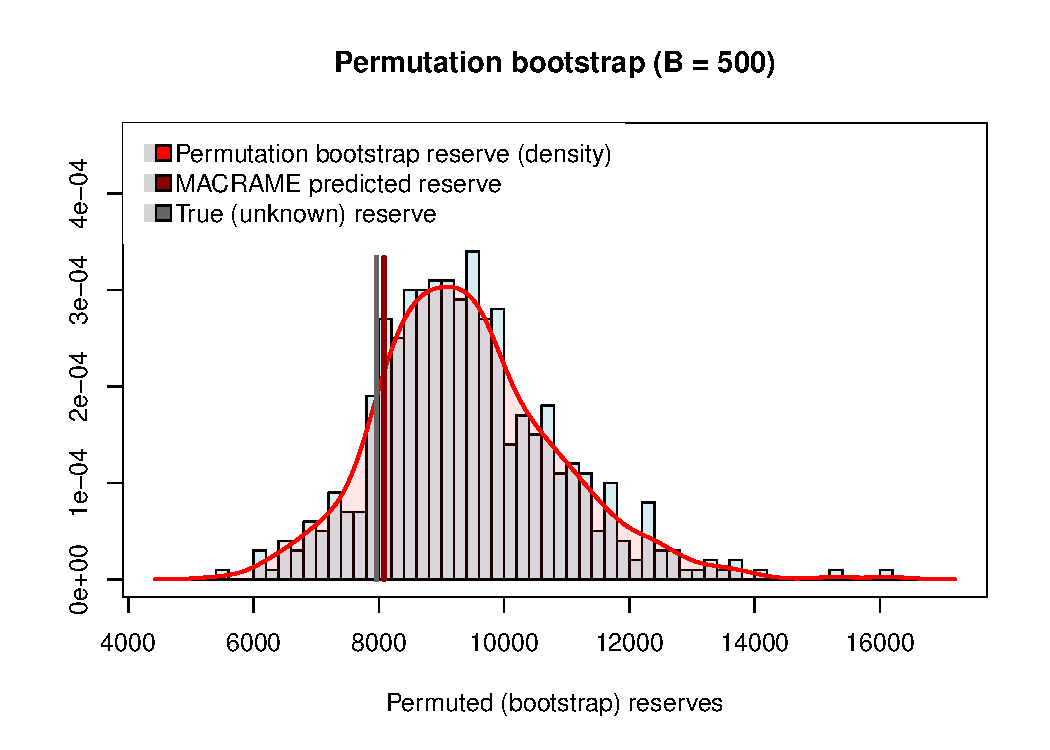
\includegraphics[width = 7.3cm]{fig8_B.pdf}
         \caption{Histogram and the estimated density}
         \label{fig10b}
    \end{subfigure}   

    \begin{subfigure}{.49\textwidth} 
            \centering
            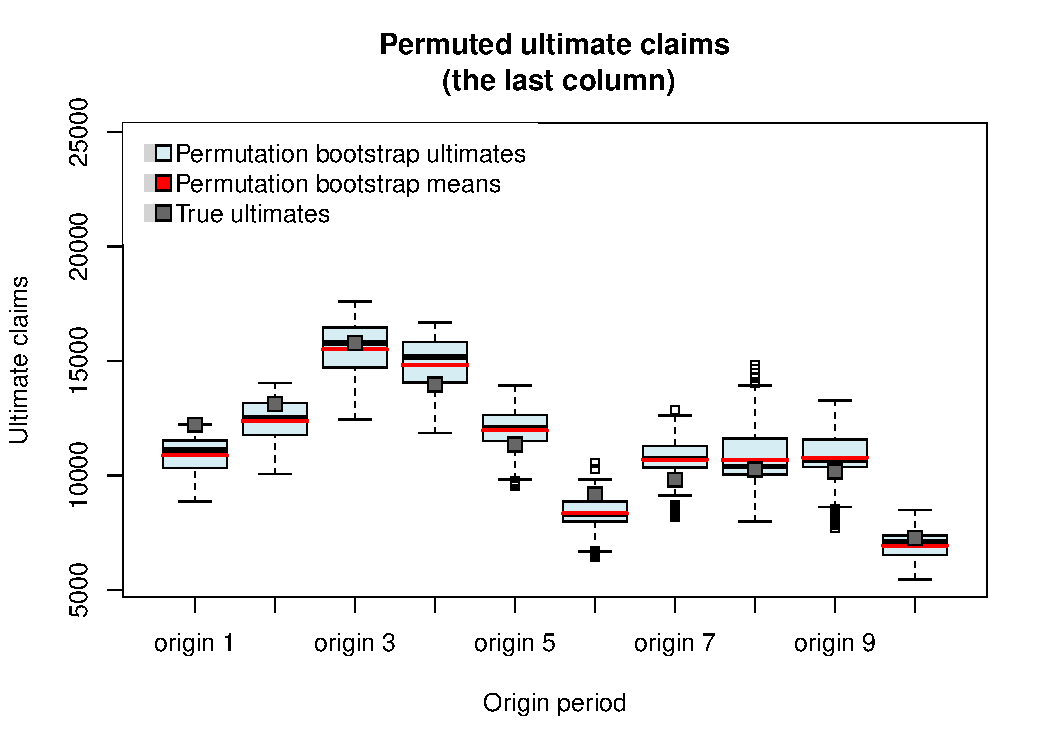
\includegraphics[width = 7.3cm]{fig8_C.pdf}
        \caption{Simulated ultimate claims}
         \label{fig10c}
    \end{subfigure}
    \begin{subfigure}{.49\textwidth} 
            \centering
        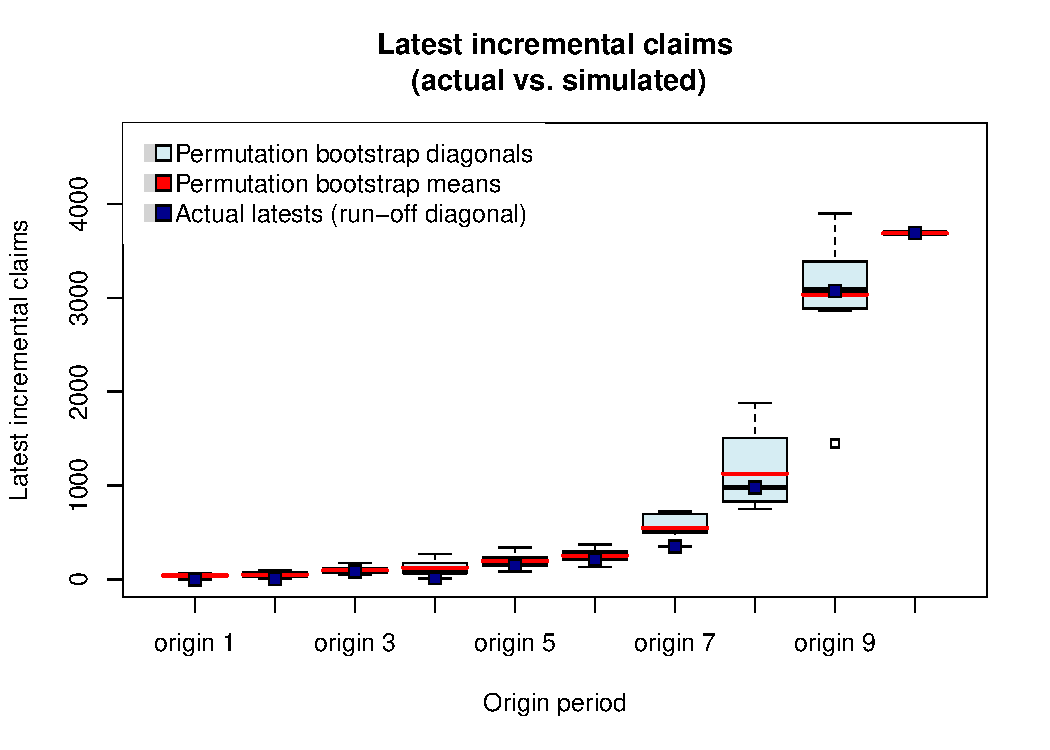
\includegraphics[width = 7.3cm]{fig8_D.pdf}
         \caption{Simulated run-off diagonals}
         \label{fig10d}
    \end{subfigure} 
    \caption{\footnotesize Graphical output of the \code{permuteReserve()} function when applied to the \code{CameronMutual} run-off triangle using the MACRAME  algorithm and $B = 500$ permutation bootstrap resamples. Four panels are provided in an analogous way as if the \code{plot()} function is applied to the output of some parametric estimation method implemented in the \CRANpkg{ChainLadder} package (see, for instance, \code{glmReserve()} or \code{MackChainLadder()}). 
    }
    \label{fig10}
\end{figure}

The \code{permuteReserve()} function can also automatically inherit the user-based settings of the Markov chain process (parameters \code{breaks} and \code{states} in the \code{mcReserve()} function in particular) or some user-specified settings needed for the parametric reserving methods (for instance, the link function used for the GLM based reserving or the Tweedie model). In case of the MACRAME algorithm, either the set of states and breaks is automatically adjusted for each permuted run-off triangle (parameter \code{adjustMC = TRUE} which is the default option) or the same set of states and breaks is used for each permuted run-off triangle (\code{adjustMC = FALSE}) and, in addition, no standardization step defined in \eqref{eq_std} is applied in such situation. The \code{permuteReserve()} function can be used analogously also for classical parametric methods---for instance, the permutation bootstrap applied to the Over-dispersed Poisson model implemented in \code{glmReserve()} from the \CRANpkg{ChainLadder} package can be obtained as 
\begin{Verbatim}[commandchars=\\\{\}]
    R> (distribution.glm <- permuteReserve(glmReserve(observed(CameronMutual))))
      |>>>>>>>>>>>>>>>>>>>>>>>>>>>>>>>>>>>>>>>>>>>| 100% elapsed=08s
    \textcolor{magenta}{MACRAME based reserving}
       Est.Reserve    Est.Ultimate     Paid Amount    True Reserve 
          8601          113760          105159              NA 
    \textcolor{magenta}{Permutation bootstrap (B = 500)}
         Boot.Mean         Std.Er.        BootCov%     BootVar.995 
          10889.391       1249.785         11.477          1.254 
\end{Verbatim}

\subsection{Computational efficiency and limitations}
\label{efficiency}
The proposed functional-based reserving methods (including the permutation bootstrap algorithm) 
are computationally very effective---particularly when compared with some classical reserving techniques 
and standard residual bootstrap implemented in the \CRANpkg{ChainLadder} package. To illustrate this efficiency and to compare the performance of the nonparametric methods (i.e., PARALLAX, REACT, and MACRAME) with parametric ones (in particular: the chainladder method implemented in \code{chainladder()}; Mack model from \code{MackChainLadder()}; over-dispersed Poisson model in \code{glmReserve()}; and Tweedie model implemented in \code{tweedieReserve()}) we used three large ($60 \times 60$) run-off triangles from the \code{GFCIB} dataset (the fourth run-off triangle---the annuities---cannot be used with the chainladder method and the Mack model due to some fully zero rows) and the point predictions were obtained together with the distributional predictions (using the permutation bootstrap for each method and the residual based bootstrap implemented in \CRANpkg{ChainLadder} 
for the ODP model (\code{glmReserve(..., mse.method = "bootstrap")})
and the Tweedie model (\code{tweedieReserve(..., bootstrap = 1)}). The number of bootstrap resamples was always set 
to $B = 1000$ and MacOS Architecture with 12 Apple M2 Pro chips (8 for performance and 4 for efficiency) with 32GB memory was used to get the results summarized in Table~\ref{efficiency_comparisons}.

\renewcommand{\arraystretch}{0.9}
\begin{table}[!t]
    \centering
    \begin{tabular}{lccc}
        \toprule
        {\bf Prediction method} & \textbf{Point prediction} & {\bf Permutation bootstrap} & {\bf Residual bootstrap} \\\midrule
        PARALLAX & $0.03s.$ \scalebox{0.8}{(0.006)} & $~15.01s.$ \scalebox{0.8}{(0.341)} & \ding{55} \\
        REACT & $0.01s.$ \scalebox{0.8}{(0.001)} & $~~~9.04s.$ \scalebox{0.8}{(0.116)} & \ding{55} \\
        MACRAME & $0.04s.$ \scalebox{0.8}{(0.012)} & $~48.75s.$ \scalebox{0.8}{(11.51)} & \ding{55} \\[0.15cm]

        Chainladder & $0.03s.$ \scalebox{0.8}{(0.008)} & $~31.70s.$ \scalebox{0.8}{(0.276)} & \ding{55} \\ 
        Mack model & $0.04s.$ \scalebox{0.8}{(0.002)} & $~42.10s.$ \scalebox{0.8}{(0.650)} & \ding{55} \\
        ODP model & $3.86s.$ \scalebox{0.8}{(0.043)} & $63.37m.$ \scalebox{0.8}{(0.148)} & $~~~\infty~m.$ \scalebox{0.8}{(NA$^{*}$)} \\
        Tweedie formula & $0.24s.$ \scalebox{0.8}{(0.026)} & $~~4.19m.$ \scalebox{0.8}{(0.307)} & $~~3.69m.$ \scalebox{0.8}{(0.252)} \\
         \bottomrule
    \end{tabular}
    \caption{\footnotesize Computational efficiency in terms of the running times for different prediction algorithms from the \CRANpkg{ProfileLadder} and \CRANpkg{ChainLadder} package. Point predictions together with distributional predictions obtained by the proposed permutation bootstrap and the classical residual bootstrap (applied only to some (available) methods from the \CRANpkg{ChainLadder} package) are compared (using $1000$ bootstrap replicates). Three run-off triangles of the dimensions $60 \times 60$ from the dataset \code{GFCIB} from \CRANpkg{ProfileLadder} are used and the running times (given either in seconds $[s.]$ or minutes $[m.]$ for brevity) are averaged (with the corresponding standard errors in brackets).\\
    $^{*}$ The residual bootstrap for the ODP model was terminated after six days of running without any results.}
    \label{efficiency_comparisons}
\end{table}

The limitations of the proposed methods are, on the other hand, mostly determined by the \CRANpkg{ChainLadder} package rather than the functions from \CRANpkg{ProfileLadder} themselves. In principle, there is no theoretical limitation for PARALLAX, REACT, or MACRAME to handle as minimal run-off triangles as $2 \times 2$. However, unlike \code{parallelReserve()} which indeed handles such cases,  \code{mcReserve()} does not (and the minimum dimensions required are $3 \times 3$). This is caused by the internal implementation of the \code{cum2incr()} function from the \CRANpkg{ChainLadder} package which transforms  cumulative triangles into incremental ones. On the other hand, there are no formal limitations for the maximum allowed dimensions that we would be aware of. 

\subsection{Other features of the R package \CRANpkg{ProfileLadder}}
\label{Raddons}
The main core of the R package \CRANpkg{ProfileLadder} consists of three key functions---\code{parallelReserve()} for applying the PARALLAX or REACT algorithm, \code{mcReserve()} implementing the MACRAME algorithm, and \code{permutedReserve()} providing the permutation bootstrap add-on. Other generic functions (for the R objects of the class \code{profileLadder}, \code{profilePredict}, \code{mcSetup}, and \code{permutedReserve}) are also implemented to facilitate a~well structured summary of the outputs and  graphical visualizations of the results. In addition, there are a few other helpful functions implemented in \CRANpkg{ProfileLadder}. For a~complex description and illustrative examples, we  refer to the R help session by using the standard \code{help()} command. Below, we only provide a~brief description of the three  most relevant functions that in some sense interconnect our package \CRANpkg{ProfileLadder} with the core actuarial package \CRANpkg{ChainLadder} and some typical insurance standards.  

\begin{itemize}[topsep=0pt, partopsep=0pt, itemsep=5pt, parsep=0pt, labelindent=0pt, leftmargin=10pt]
    \item \code{as.profileLadder()}
    \indent For the run-off triangle data type there is already an R class \code{triangle} implemented in the R package \CRANpkg{ChainLadder} by \cite{Rchainladder} with the corresponding R function \code{as.triangle()}. This is a generic {S3} class method that eases the work with the triangle shaped matrix data. However, the generic summary and plot methods do not allow distinguishing the observed functional profiles and the unknown ``future'' segments when using this R class. Therefore, we introduce an enhanced run-off triangle class \code{profileLadder} that provides more appropriate organization suitable for the nonparametric functional-based reserving techniques. For illustration, compare the following R code that produces two plots in Figure~\ref{fig9}. 

    \begin{verbatim}
    ### S3 class 'triangle' from the ChainLadder pkg
    R> plot(as.triangle(CameronMutual))

    ### S3 class 'profileLadder' from the ProfileLadder pkg
    R> plot(as.profileLadder(CameronMutual))
    \end{verbatim}
    The new R class \code{ProfileLadder} also provides some additional information about the underlying run-off triangle (for instance, the true reserve amount if available, the triangle type--cumulative or incremental---and way more) and it also adapts various information provided by the functional-based algorithms (PARALLAX, REACT, or MACRAME);
    \begin{figure}[!t]
        \begin{subfigure}{.49\textwidth} 
            \centering
            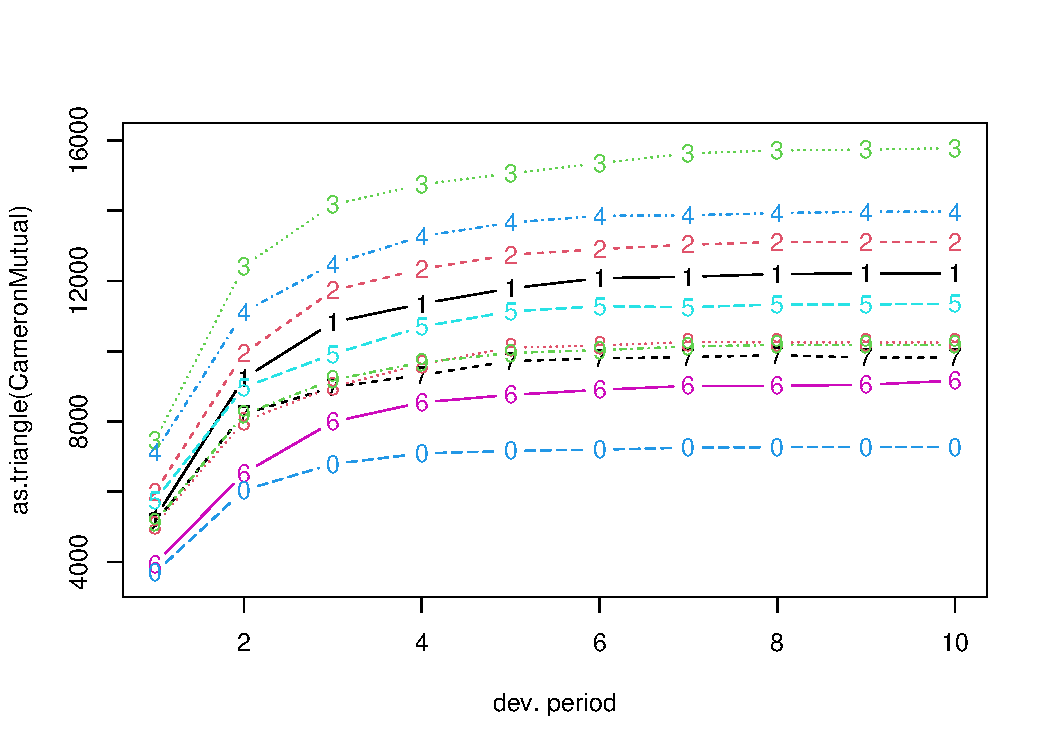
\includegraphics[width = 7.5cm]{fig9_A.pdf}
        \caption{\code{plot(as.triangle(CameronMutual))}}
         \label{fig9a}
    \end{subfigure}
    \begin{subfigure}{.49\textwidth} 
            \centering
        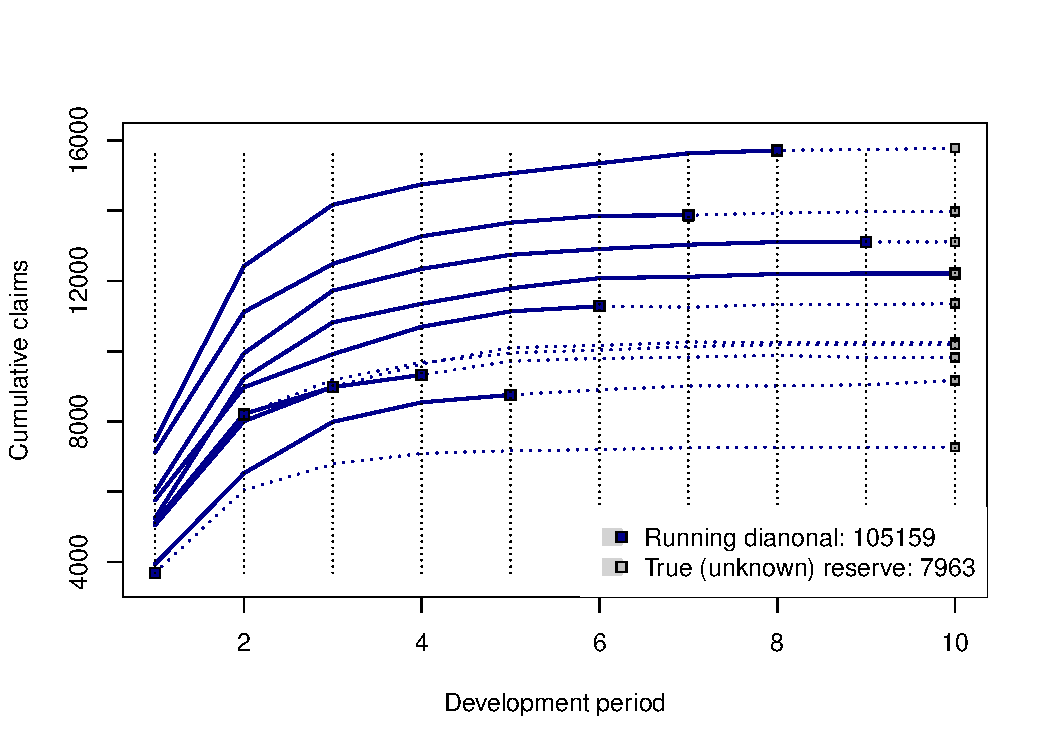
\includegraphics[width = 7.5cm]{fig9_B.pdf}
         \caption{\code{plot(as.profileLadder(CameronMutual))}}
         \label{fig9b}
    \end{subfigure}   
    \caption{\footnotesize Graphical comparison of the performance of the generic R method \code{plot()} when applied to the same data set (\code{CameronMutual}) represented by different R classes. The left-hand panel shows the result for the \code{triangle} class defined in the package \CRANpkg{ChainLadder}; the result for the \code{profileLadder} class is shown on the right-hand side.}
    \label{fig9}
\end{figure}

    \item \code{observed()} This function provides practical layouts (of different types) to distinguish observed and un\-ob\-served functional profiles in the run-off triangle (mainly in situations when the triangle is provided in terms of a full data matrix). This R function 
    also allows for an application of classical reserving approaches from the \CRANpkg{ChainLadder} package (such as the \code{glmReserve()}, \code{tweedieReserve()}, or \code{MackChainLadder()}) to be easily used with the fully observed run-off triangles supplemented in the \CRANpkg{ProfileLadder} package. The run-off triangles included as example datasets in the \CRANpkg{ProfileLadder} package are (mostly) given in terms of full (squared) matrices (with the ``unknown'' future development profiles being also provided for an ex-post performance evaluation) while the parametric methods implemented in the \CRANpkg{ChainLadder} package rely solely on the input data in  form of the run-off triangle---meaning that $Y_{i,j} = X_{i,j} = \textrm{\code{NA}}$ for all $i + j > n + 1$.  Compare, for instance, the following (where the first command results in an error message while the latter already works properly): 
    \begin{verbatim}
    R> glmReserve(CameronMutual)
    R> glmReserve(observed(CameronMutual))
    \end{verbatim}
    The same reasoning also applies for other parametric reserving methods from the \CRANpkg{ChainLadder} package (\code{tweedieModel()} and \code{MackChainLadder()} functions in particular).

    \item \code{predict()}  A generic S3 class method applicable to the outputs of the \code{parallelReserve()} function and the \code{mcReserve()} function---the objects of the class \code{profileLadder}. For internal purposes of insurance companies, actuaries are at times interested in a~one-step-ahead prediction only (typically a 1-year-ahead prediction say). Instead of completing the run-off triangle into a full square, the focus is then on predicting the so-called \emph{next running diagonal}. The S3 method \code{predict.profileLadder()} performs this as
    \begin{verbatim}
    R> predict(parallelReserve(CameronMutual))
    \end{verbatim}
    Unlike the run-off triangle completion where the output of \code{parallelReserve()} or \code{mcReserve()} is a matrix of the dimensions $n \times n$, the output of the \code{predict()} method is actually a~new run-off triangle of the dimensions $n \times (n + 1)$ (the output is omitted for brevity).
\end{itemize}

\section{Concluding remarks and summary}
\label{beyondSection}
The \CRANpkg{ProfileLadder} package is particularly developed to implement nonparametric methods into the actuarial risk assessment process performed by insurance companies (typically on~a~yearly or quarterly basis). Nevertheless, the underlying run-off triangle can be formally also represented in terms of an incomplete panel data scheme  that is generally well known among statisticians and all types of practitioners. 
%The triangular shaped data are  common in many areas where cumulative data is observed over time.
The statistical techniques and specific functions implemented in the R package \CRANpkg{ProfileLadder} can be also used for such data. Some explicit datasets (briefly described below) are included in the package to illustrate possible applications beyond the actuarial domain.

\begin{itemize}[topsep=0pt, partopsep=0pt, itemsep=0pt, parsep=0pt, labelindent=0pt, leftmargin=10pt]
    \item \textbf{Health care \& epidemiology} 
    Triangular data, similar to run-off triangles, are common in tracking medical claims and receipts until resolution. Another example is epidemiological monitoring, such as tracking disease spread by new cases in specific cohorts over time. The dataset \code{covid19CZ} (see \code{help("covid19CZ")}) captures the spread of Covid-19 in Czechia over the first eight weeks using weekly cohort data by counties (grouped by the week of the first case occurrence). We use also this data to demonstrate the functionality of the \code{predict()} method mentioned at the end of the previous section. This function is not only useful for the actuaries, but it also has important practical utilization in any type of risk modeling. The S3 method \code{predict()} is implemented for the objects of the R class \code{profileLadder} that are created by the \code{parallelReserve()} function or the \code{mcReserve()} function (for details, we refer to the help session obtained by \code{help("predict.profileLadder")}).

    Instead of completing the run-off triangle into a full square (by one of the algorithms PARALLAX, REACT, or MACRAME), the \code{predict()} method only returns the prediction of the next running diagonal (also called a \emph{1-step-ahead prediction}). The same algorithms are used for the diagonal prediction, only the output is not a completed square but rather a new (extended) run-off triangle of the dimensions $n \times (n + 1)$.

    For illustration, the \code{predict()} method is applied below to the run-off triangle formed from the dataset \code{covid19CZ}, using all four cohorts (rows) and weeks 3 to 6 (i.e., columns 3 to 6), to allow for an ex post comparison between the diagonal prediction and the actual true outcome (the next running diagonal in \code{covid19CZ}).
        The output from the \code{predict()} method is another object of the R class \code{profilePredict} with the corresponding plot method, which provides a graphical illustration---see the R code and Figure~\ref{fig:covid19} below.

\begin{figure}[htbp]
\centering
\hspace*{0.5cm}
\begin{minipage}{0.6\textwidth}
\small 
\begin{Verbatim}[commandchars=\\\{\}]

R> diagonal <- predict(mcReserve(covid19CZ[,3:6]))
R> print(diagonal)

  01/03 - 07/03     392   676  1158  1366  \textcolor{magenta}{1396} 	
  08/03 - 14/03    1126  1702  2058  \textcolor{magenta}{2264     .}
  15/03 - 21/03     970  1173  \textcolor{magenta}{1173     .     .}	
  22/03 - 28/03     164   \textcolor{magenta}{164     .     .     .}

R> plot(diagonal, trueProfiles = covid19CZ[,1:7])
\end{Verbatim}
\end{minipage}%
\hfill
\begin{minipage}{0.35\textwidth}
\centering\vskip-0.5cm
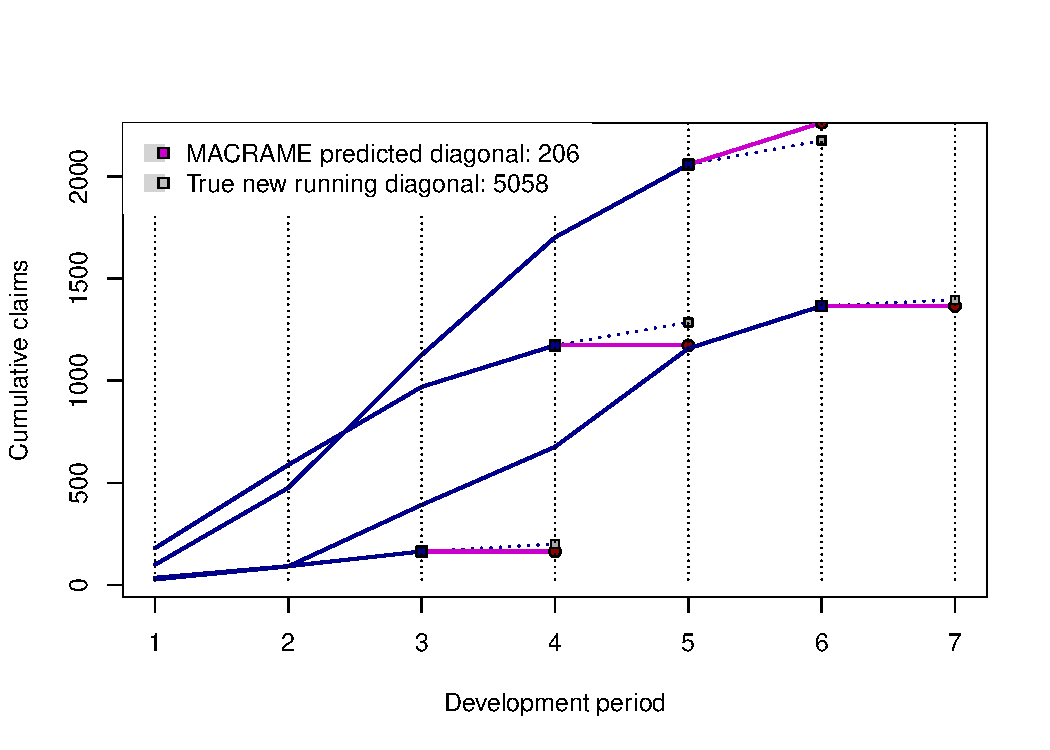
\includegraphics[width=1.0\linewidth]{fig10.pdf}
\caption{\footnotesize 1-step-ahead prediction}
\label{fig:covid19}
\end{minipage}
\end{figure}
Moreover, the S3 method \code{predict()} can be  applied repeatedly to predict other consecutive diagonals as the output of the \code{predict()} function is a run-off triangle (although of a rectangular shape with dimensions $n \times (n + 1)$), and, thus, it can be forwarded again as the input for \code{parallelReserve()} or \code{mcReserve()} (considering all $n$ rows but only  last $n$ columns).

    \item \textbf{Accounting \& auditing} 
    Tracking unpaid invoices or tax adjustments based on past years is common in business and government, and such data often form a triangle structure too. The dataset \code{xNetSubscribe} (see \code{help("xNetSubscribe")}) illustrates this with monthly income from a local internet provider, using cohorts of new subscribers by month;

    \item \textbf{Operational risk \& banking} 
        In general, the occurrence and development of events like fraud, IT failures, or compliance breaches can be viewed through the lens of operational risk. Such events are often tracked using development triangles, with rows indicating occurrence time and columns showing development periods;

    \item \textbf{Manufacturing \& quality control} Triangular data also arise in various production processes. The triangular schemes are typically generated when tracking defects and failures within specific production batches in order to  predict failure rates and to manage maintenance schedules.
\end{itemize}
From the overall point of view, the nonparametric point prediction methods implemented in the R package \CRANpkg{ProfileLadder} (the algorithms PARALLAX, REACT, and MACRAME) are, despite the fact that all were developed specifically for the claims reserving purposes, widely applicable to any triangular data schemes arising in real-life applications. There are three core functions in the package: the first one, \code{parallelReserve()}, implements the PARALLAX algorithm and the REACT algorithm; the second one, \code{mcReserve()}, incorporates a more complex Markov chain prediction mechanism with a~whole variety of user-based options; the third function, \code{permuteReserve()}, estimates for the overall reserve distribution---not exclusively for the proposed functional-based methods, but also for classical parametric reserving approaches. This function may thus serve as a practical alternative to a parametric (residual) bootstrap. Auxiliary R functions are also implemented to make the work with the  triangular shaped data easier and more straightforward especially when interacting with the actuarial package \CRANpkg{ChainLadder}. Finally, unique illustrative datasets from the actuarial practice and other practical real-world areas are featured as well.  

\newpage

\noindent \textbf{Acknowledgment}
\footnotesize
The work of Maciak, Mizera, and Pe\v{s}ta was supported by the Czech Science Foundation grant  GAČR~23--06461K. The work of Matúš was supported by MSD Czech Republic.  The work of Maciak was also partially
supported by COST (European
Cooperation in Science and Technology)
— COST Action HiTEc, No. CA21163. 
The authors express sincere thanks to Kurt Hornik for his insight and some useful pieces of advice regarding the \CRANpkg{ProfileLadder} package. The authors are also grateful to Petr Jedlička from the Czech Insurers’ Bureau and Pavel Koudelka from Generali Česká pojišť\hspace{-0.04cm}ovna for providing complex data from real-life insurance practice---not only for internal evaluation purposes but also for public access within the R~package \CRANpkg{ProfileLadder}. Last but not least, the authors appreciate the insight and help of Rob Hyndman and two anonymous reviewers---particularly for their suggestions and comments that helped to improve the overall quality of the package and the manuscript. The authors declare no conflict of interest.

\setlength{\bibsep}{2.8pt}

% Bibliography
\bibliography{MMMP}

\smallskip

\parbox[t]{0.60\textwidth}{
  \textbf{Matúš Maciak}, \textbf{Ivan Mizera}, \textbf{Michal Pešta} \\[0.1cm]
  Charles University, Faculty of Mathematics and Physics\\
  Sokolovská~49/83, Prague, 186~00\\
  Czech Republic\\[0.1cm]
  \email{maciak|mizera|pesta@karlin.mff.cuni.cz}%\\
}
\hfill
\parbox[t]{0.40\textwidth}{
  \textbf{Rastislav Matúš} \\[0.1cm]
  Merck Sharp \& Dohme s.r.o.\\
  Na Valentince 3336/4, Prague, 150~00\\
  Czech Republic\\[0.1cm]
  \email{rastislav.matus@merck.com}
}

\end{article}

\end{document}
